% Options for packages loaded elsewhere
% Options for packages loaded elsewhere
\PassOptionsToPackage{unicode}{hyperref}
\PassOptionsToPackage{hyphens}{url}
\PassOptionsToPackage{dvipsnames,svgnames,x11names}{xcolor}
%
\documentclass[
  french,
  11pt,
  a4paper,
]{article}
\usepackage{xcolor}
\usepackage[top=1.5cm, bottom=1.5cm, left=2.5cm, right=2.5cm]{geometry}
\usepackage{amsmath,amssymb}
\setcounter{secnumdepth}{5}
\usepackage{iftex}
\ifPDFTeX
  \usepackage[T1]{fontenc}
  \usepackage[utf8]{inputenc}
  \usepackage{textcomp} % provide euro and other symbols
\else % if luatex or xetex
  \usepackage{unicode-math} % this also loads fontspec
  \defaultfontfeatures{Scale=MatchLowercase}
  \defaultfontfeatures[\rmfamily]{Ligatures=TeX,Scale=1}
\fi
\usepackage{lmodern}
\ifPDFTeX\else
  % xetex/luatex font selection
  \setmainfont[]{TeX Gyre Termes}
\fi
% Use upquote if available, for straight quotes in verbatim environments
\IfFileExists{upquote.sty}{\usepackage{upquote}}{}
\IfFileExists{microtype.sty}{% use microtype if available
  \usepackage[]{microtype}
  \UseMicrotypeSet[protrusion]{basicmath} % disable protrusion for tt fonts
}{}
\makeatletter
\@ifundefined{KOMAClassName}{% if non-KOMA class
  \IfFileExists{parskip.sty}{%
    \usepackage{parskip}
  }{% else
    \setlength{\parindent}{0pt}
    \setlength{\parskip}{6pt plus 2pt minus 1pt}}
}{% if KOMA class
  \KOMAoptions{parskip=half}}
\makeatother
% Make \paragraph and \subparagraph free-standing
\makeatletter
\ifx\paragraph\undefined\else
  \let\oldparagraph\paragraph
  \renewcommand{\paragraph}{
    \@ifstar
      \xxxParagraphStar
      \xxxParagraphNoStar
  }
  \newcommand{\xxxParagraphStar}[1]{\oldparagraph*{#1}\mbox{}}
  \newcommand{\xxxParagraphNoStar}[1]{\oldparagraph{#1}\mbox{}}
\fi
\ifx\subparagraph\undefined\else
  \let\oldsubparagraph\subparagraph
  \renewcommand{\subparagraph}{
    \@ifstar
      \xxxSubParagraphStar
      \xxxSubParagraphNoStar
  }
  \newcommand{\xxxSubParagraphStar}[1]{\oldsubparagraph*{#1}\mbox{}}
  \newcommand{\xxxSubParagraphNoStar}[1]{\oldsubparagraph{#1}\mbox{}}
\fi
\makeatother


\usepackage{longtable,booktabs,array}
\newcounter{none} % for unnumbered tables
\usepackage{calc} % for calculating minipage widths
% Correct order of tables after \paragraph or \subparagraph
\usepackage{etoolbox}
\makeatletter
\patchcmd\longtable{\par}{\if@noskipsec\mbox{}\fi\par}{}{}
\makeatother
% Allow footnotes in longtable head/foot
\IfFileExists{footnotehyper.sty}{\usepackage{footnotehyper}}{\usepackage{footnote}}
\makesavenoteenv{longtable}
\usepackage{graphicx}
\makeatletter
\newsavebox\pandoc@box
\newcommand*\pandocbounded[1]{% scales image to fit in text height/width
  \sbox\pandoc@box{#1}%
  \Gscale@div\@tempa{\textheight}{\dimexpr\ht\pandoc@box+\dp\pandoc@box\relax}%
  \Gscale@div\@tempb{\linewidth}{\wd\pandoc@box}%
  \ifdim\@tempb\p@<\@tempa\p@\let\@tempa\@tempb\fi% select the smaller of both
  \ifdim\@tempa\p@<\p@\scalebox{\@tempa}{\usebox\pandoc@box}%
  \else\usebox{\pandoc@box}%
  \fi%
}
% Set default figure placement to htbp
\def\fps@figure{htbp}
\makeatother



\ifLuaTeX
\usepackage[bidi=basic,shorthands=off]{babel}
\else
\usepackage[bidi=default,shorthands=off]{babel}
\fi
\ifPDFTeX
\else
\babelfont{rm}[]{TeX Gyre Termes}
\fi
\ifLuaTeX
  \usepackage{selnolig} % disable illegal ligatures
\fi


\setlength{\emergencystretch}{3em} % prevent overfull lines

\providecommand{\tightlist}{%
  \setlength{\itemsep}{0pt}\setlength{\parskip}{0pt}}



 


\usepackage{enumitem}
\setlist[itemize]{label=$\bullet$}  % Puce ronde classique
\usepackage{amsmath, amssymb}
\makeatletter
\@ifpackageloaded{caption}{}{\usepackage{caption}}
\AtBeginDocument{%
\ifdefined\contentsname
  \renewcommand*\contentsname{Table des matières}
\else
  \newcommand\contentsname{Table des matières}
\fi
\ifdefined\listfigurename
  \renewcommand*\listfigurename{Liste des Figures}
\else
  \newcommand\listfigurename{Liste des Figures}
\fi
\ifdefined\listtablename
  \renewcommand*\listtablename{Liste des Tables}
\else
  \newcommand\listtablename{Liste des Tables}
\fi
\ifdefined\figurename
  \renewcommand*\figurename{Figure}
\else
  \newcommand\figurename{Figure}
\fi
\ifdefined\tablename
  \renewcommand*\tablename{Table}
\else
  \newcommand\tablename{Table}
\fi
}
\@ifpackageloaded{float}{}{\usepackage{float}}
\floatstyle{ruled}
\@ifundefined{c@chapter}{\newfloat{codelisting}{h}{lop}}{\newfloat{codelisting}{h}{lop}[chapter]}
\floatname{codelisting}{Listing}
\newcommand*\listoflistings{\listof{codelisting}{Liste des Listings}}
\makeatother
\makeatletter
\makeatother
\makeatletter
\@ifpackageloaded{caption}{}{\usepackage{caption}}
\@ifpackageloaded{subcaption}{}{\usepackage{subcaption}}
\makeatother
\usepackage{bookmark}
\IfFileExists{xurl.sty}{\usepackage{xurl}}{} % add URL line breaks if available
\urlstyle{same}
% fallback for those not using the hyperref driver hyperxmp:
\makeatletter
\@ifundefined{xmpquote}{\newcommand{\xmpquote}[1]{#1}}{}
\makeatother
\hypersetup{
  pdflang={fr},
  colorlinks=true,
  linkcolor={blue},
  filecolor={Maroon},
  citecolor={Blue},
  urlcolor={Blue},
  pdfcreator={LaTeX via pandoc}}


\author{}
\date{}
\begin{document}


\begin{titlepage}
\raggedright


\includegraphics{../ressources/ensai_logo_2.png}\\

\centering
\vspace{0.5cm}
{\LARGE\textsc{Rapport de projet VeloScope}}\\
\vspace{0.5cm}

\vspace{1.5cm}

\rule{\textwidth}{0.5mm}\\
\vspace{0.8cm}
{\huge\bfseries VeloScope}\\
\vspace{0.8cm}
\rule{\textwidth}{0.5mm}\\

\vspace{1.5cm}

\begin{flushleft}
\emph{Étudiant·e·s :}\\
Fanny BOUBY\\
Audrey DANJOIE\\
Romane DELANZY\\
Jean POHARDY\\
Elouan REGUIGNE GRANCHER\\
\end{flushleft}

\begin{flushright}
\emph{Responsable :}\\
Ludovic DENEUVILLE\\
\vspace{0.5cm}
\emph{Tuteur :}\\
André RIVIERE\\
\end{flushright}


\vfill 
\begin{center}
École nationale de la statistique et de l’analyse de l’information\\
2026--2027
\end{center}
\end{titlepage}

\tableofcontents

\pagebreak

\section{Introduction}\label{introduction}

\subsection{Remise en contexte et
problématique}\label{remise-en-contexte-et-probluxe9matique}

Dans un contexte de transition écologique et de décongestion des centres
urbains, l'encouragement à l'usage du vélo au quotidien est devenu une
priorité majeure pour les collectivités. Les réseaux de vélos en
libre-service jouent un rôle clé dans cette dynamique de mobilité douce.
Aujourd'hui, la plupart des métropoles mettent à disposition des
applications mobiles affichant une carte des stations en temps réel. Son
usage reste pourtant soumis à certaines incertitudes. Par exemple, on ne
sait pas si l'on trouvera un vélo ou une place libre pour rendre un vélo
lorsqu'on arrivera à une station. Les réseaux publient la disponibilité
à l'instant présent, mais cette information ne dit rien de la régularité
d'une station : certaines sont fréquemment vides aux heures de pointe ou
saturées le soir, d'autres sont presque toujours utilisables.

Comment dépasser la simple visualisation instantanée de l'état d'un
réseau de vélos en libre-service pour fournir aux usagers des
indicateurs historiques de fiabilité et des recommandations
personnalisées fiables ?

Notre réponse avec VeloScope : Contrairement aux applications classiques
qui affichent l'état du réseau à la dernière date de relevé seulement,
VeloScope construit sa propre mémoire. Notre application interroge
périodiquement les serveurs de données publiques de la ville de Bordeaux
(VLS Le Vélo TBM Bordeaux Métropole) et historise chaque relevé dans une
base de données. En analysant cet historique, VeloScope calcule des
indicateurs de performance (taux de pénurie, taux de saturation, score
de fiabilité) et propose un moteur de recommandation multicritère aidant
l'usager à choisir la station la plus pertinente.

Sera décrit dans ce rapport le nécessaire pour connaître le
fonctionnement de l'application : fonctionnalités, données utilisées,
architecture de l'application, rapport de tests qualité. Nous détaillons
en particulier la fonctionnalité principale de recommandation de
stations dans la partie ``Réponse aux besoins''.

\subsection{A qui s'adresse
l'application?}\label{a-qui-sadresse-lapplication}

~~~~~~~~

VeloScope s'adresse à deux profils d'utilisateurs distincts, structurés
selon un principe d'héritage des droits afin de simplifier l'usage
quotidien :

\begin{itemize}
\item
  L'Usager du réseau (Utilisateur standard) : Il représente tout
  citoyen, étudiant ou travailleur souhaitant optimiser ses déplacements
  à vélo en ville. Après avoir créé son compte personnel et s'être
  connecté, il peut rechercher une station, visualiser l'évolution de sa
  disponibilité sur différentes périodes (24h, 7 jours, 30 jours),
  consulter son score de fiabilité, enregistrer ses stations habituelles
  en favoris, explorer la carte interactive du réseau ou demander une
  recommandation de station et d'itinéraire. Une liste de toutes les
  stations de vélo de la ville de Bordeaux lui est également disponible.
\item
  L'Administrateur : Il s'agit du gestionnaire technique de la
  plateforme. Il dispose exactement des mêmes fonctionnalités qu'un
  usager standard (il n'a donc pas besoin de jongler entre deux comptes
  distincts pour utiliser l'application), mais bénéficie en plus d'un
  espace d'administration lui permettant de superviser les comptes
  inscrits. Il peut ainsi accéder à la liste de tous les utilisateurs,
  modifier les informations d'un compte si nécessaire (nom d'utiliateur,
  email, mot de passe, droits administrateur), ou supprimer un compte.
  Ce profil s'adresse principalement aux techniciens de maintenance et
  développeurs, dans le cas par exemple où un utilisateur aurait oublié
  son mot de passe. Notons que nous n'avons volontairement pas donné de
  droits sur la base de données à l'administrateur afin de préserver son
  intégrité. La gestion de cette base est faite automatiquement grâce au
  système de collecte présent en arrière plan de manière permanente dans
  notre application.
\end{itemize}

\pagebreak

\section{Présentation générale}\label{pruxe9sentation-guxe9nuxe9rale}

\subsection{Organisation du groupe et gestion du
projet}\label{organisation-du-groupe-et-gestion-du-projet}

Pour mener à bien ce projet sur une durée de trois mois (de septembre à
novembre 2026), notre équipe de cinq étudiants a adopté l'organisation
suivante. Nous devions à la fois répartir les différentes tâches dans le
temps et entre les membres du groupe.

Pour ce faire, nous avons, dès le début du projet organisé les grandes
phases de notre travail dans le temps grâce à un diagramme de Gantt. Il
nous a permit de découper le projet en 2 temps. Une première phase de
conception en septembre dont les objectifs principaux étaient: la
compréhension du sujet, la recherche de bases de données, la réflexion
sur la structure de l'application et les réalisations des différents
graphiques. La deuxième phase a débuté après le rendu du rapport
intermédiaire. Elle était centrée sur la construction progressive et
incrémentable de l'application via l'écriture du code.

\pandocbounded{\includegraphics[keepaspectratio,alt={Diagramme de Gantt du Rapport d'Analyse}]{../ressources/Diagramme/Diagramme_gantt1.png}}
\pandocbounded{\includegraphics[keepaspectratio,alt={Diagramme de Gantt du Code et du Rapport Final}]{../ressources/Diagramme/Diagramme_gantt2.png}}

D'autre part, nous avons essayé de nous réunir assez régulièrement pour
nous répartir les différentes tâches et faire le point sur ce qui avait
été fait. La répartition des tâches s'est faite de manière à ce que
chaque membre puisse toucher à un élément de chaque couche de
l'application. Ainsi, chaque membre a participé a codé au moins un
business object, un DAO, un controller et un service. Nous avons essayé
de tenir compte au mieux des atouts et des préferences de chacun dans la
répartition des tâches.

Ainsi, les élèves ayant davantage de facilités en informatique se sont
concentrés sur le code des classes les plus complexes
(authentification/gestion des comptes, collecte depuis l'API externe,
recommandation de station et calcul de fiabilité).

Chaque semaine jusqu'aux 3 jours de code intensif était consacrée au
code d'une couche de l'application, dans l'ordre suivant : business
object, DAO, services, controller. Nous testions l'intégralité des
classes de chaque couche avant de passer à la suivante afin de ne pas
rencontrer de problème lors du raccordement final.

L'ensemble du code a été versionné sur un dépôt GitHub commun
garantissant ainsi la cohérence et la qualité du code produit.

\subsection{Fonctionnalités de l'API et besoins
couverts}\label{fonctionnalituxe9s-de-lapi-et-besoins-couverts}

Le sujet imposait de construire une API qui collecte, historise et
analyse les données d'un réseau de vélos en libre-service. Nous l'avons
complétée par un site web interactif pour l'utilisateur avec Streamlit,
qui est le point d'accès des utilisateurs : ils y créent un compte, se
connectent, consultent les stations et demandent des recommandations,
sans appeler l'API directement.

Cinq fonctionnalités obligatoires ont été implémentées. Elles sont
détaillées ci-dessous.

\begin{itemize}
\item
  \textbf{F1 : Gestion des utilisateurs.} Un utilisateur peut créer un
  compte, se connecter et gérer ses stations favorites (ajout,
  suppression ou consultation de favoris). Un compte administrateur peut
  en plus gérer les comptes des autres utilisateurs. Chaque requête
  protégée est identifiée par un jeton transmis dans l'en-tête
  X-Auth-Token, et un champ is\_admin porté par le compte distingue les
  deux profils.
\item
  \textbf{F2 : Collecte des données.} L'API GBFS du réseau de Bordeaux
  n'expose que l'état présent des stations. Un script de collecte,
  pouvant être déclenché ou non (sur choix de l'utilisateur) lors du
  lancement de notre application, l'interroge toutes les 1h. À chaque
  passage, il met à jour la liste des stations (nom, adresse,
  coordonnées, capacité), puis enregistre un nouveau relevé de statut
  par station s'il n'a pas déjà été enregistré lors d'une précédente
  collecte : vélos disponibles (dont électriques), places libres,
  station installée, emprunt et retour autorisés. Chaque relevé est
  ajouté sans écraser les précédents, ce qui permet de reconstruire
  l'état du réseau à n'importe quel instant passé.
\item
  \textbf{F3 : Consultation d'une station.} L'utilisateur recherche une
  station par son nom et consulte son état (disponible, vide, saturée ou
  non opérationnelle), son nombre de vélos et de places disponibles, sa
  capacité et son taux de remplissage (part des places occupées). Il
  peut visualiser l'évolution de sa disponibilité sur les dernières 24
  heures, les 7 derniers jours ou les 30 derniers jours.
\item
  \textbf{F4 : Score de fiabilité.} Pour chaque station, l'application
  calcule à partir de l'historique de ses statuts le pourcentage de
  temps passé vide et saturée, la durée moyenne des périodes de vide et
  de saturation, et un score global de fiabilité tenant compte de ces
  critères compris entre 0 et 1.
\end{itemize}

Pour une station donnée, on note :

\begin{itemize}
  \item $T$ la durée totale de l'historique (en heures) ;
  \item $p_v$ la part du temps passée vide, c'est-à-dire
        la somme des durées des périodes de vide divisée par $T$ ;
  \item $p_s$ la part du temps passée saturée, c'est-à-dire
        la somme des durées des périodes de saturation divisée par $T$ ;
  \item $\bar{d}_v$ la durée moyenne, en heures, des épisodes de vide;
  \item $\bar{d}_s$ la durée moyenne, en heures, des épisodes de saturation;
  \item $c \in \{0, 1\}$ l'état actuel : $c = 1$ si la station n'est ni vide ni saturée,
        $c = 0$ sinon.
\end{itemize}

Le score de fiabilité \(S \in [0, 1]\) est la moyenne de cinq
composantes : \begin{equation}
  S = \frac{1}{5}\left[\, c + (1 - p_v) + (1 - p_s)
      + \left(1 - \frac{\bar{d}_v}{T}\right)
      + \left(1 - \frac{\bar{d}_s}{T}\right) \right]
\end{equation}

L'évolution du score dans le temps est également disponible. Il est
calculé pour chaque date disponible dans l'historique de la base de
donnée depuis la date la plus ancienne de l'historique.

\begin{itemize}
\tightlist
\item
  \textbf{F5 : Recommandation de station.} L'utilisateur saisit une
  adresse à Bordeaux, le nombre maximum de stations souhaité à
  recommander ainsi qu'un rayon de recherche. L'application convertit
  l'adresse en coordonnées, écarte les stations qui ne sont pas
  utilisables à la date du relevé le plus récent (non installée, emprunt
  impossible, aucun vélo disponible), puis classe les autres selon un
  score de recommandation égal à
\end{itemize}

\begin{equation}
  S = 0,5 \times \textrm{proximité} + 0,5 \times \textrm{fiabilité}
\end{equation}

Le score de proximité décroît avec la distance, et la fiabilité est le
score décrit dans F4. Deux stations à distance équivalente ne sont donc
pas classées de la même façon si leur score de fiabilité diffère. Le
nombre de vélos électriques disponibles et la tendance récente
(fiabilité que jusqu'à une certaine date par ex.), cités dans le sujet
comme critères possibles, ne sont pas pris en compte dans le classement.
Leur prise en compte pourrait être une source d'amélioration de ce
score.

\subsection{Les données de
l'application}\label{les-donnuxe9es-de-lapplication}

L'application VéloScope s'appuie sur des données ouvertes pour
fonctionner. Nous avons choisis d'utiliser celles fournies par la
métropole de Bordeaux concernant son réseau de vélos en libre-service
(TBM). C'était pour nous la base de donnée la plus complète compte-tenu
des fonctionnalités que nous avions à développer, ayant un nombre
raisonnable de stations (232). Son détail est disponible à l'adresse :
https://bdx.mecatran.com/utw/ws/gbfs/bordeaux/v3/gbfs.json?apiKey=opendata-bordeaux-metropole-flux-gtfs-rt

Les données externes sont récupérées via Internet au format JSON. C'est
un format texte léger et structuré très répandu pour l'échange de
données entre serveurs. Les données sur les systèmes de vélo en libre
service sont stockées selon le standard international GBFS (General
Bikeshare Feed Specification).

\begin{figure}[H]

{\centering \pandocbounded{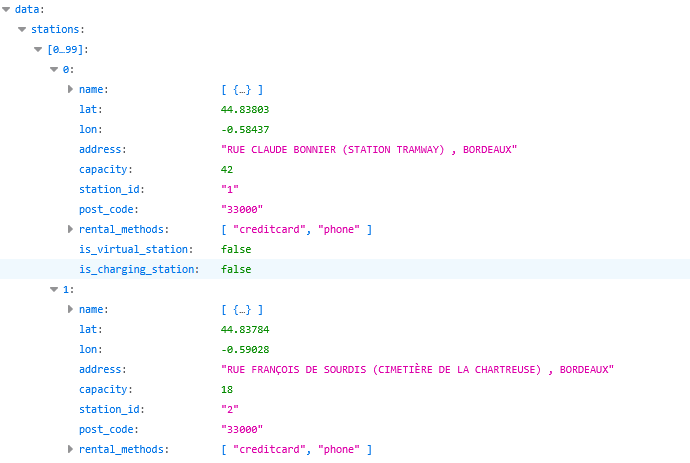
\includegraphics[keepaspectratio]{../ressources/Diagramme/json_bordeaux.PNG}}

}

\caption{Exemple de station au format JSON}

\end{figure}%

Ce standard sépare les informations en deux flux bien distincts :

\begin{itemize}
\item
  Les données statiques (station\_information) : Elles décrivent
  l'infrastructure fixe du réseau, qui change très rarement. On y trouve
  l'identifiant unique de chaque station, son nom, son adresse postale,
  sa capacité totale et ses coordonnées géographiques (latitude et
  longitude au format décimal WGS84).
\item
  Les données dynamiques (station\_status) : Elles reflètent l'activité
  du réseau en temps réel. Ce fichier contient, pour chaque identifiant
  de station, l'horodatage de la dernière mise à jour, le nombre de
  vélos mécaniques disponibles, le nombre de vélos à assistance
  électrique disponibles, le nombre de bornes libres, ainsi que des
  indicateurs booléens précisant si la station est ouverte, si l'on peut
  y louer un vélo et si l'on peut y en déposer un.
\end{itemize}

Certaines des données présentes dans l'API externe n'ont pas été
collectées, comme la méthode de rente pour chaque station, car elles
n'ont pas été jugées utiles à la réponse aux besoins.

{\def\LTcaptype{none} % do not increment counter
\begin{longtable}[]{@{}
  >{\raggedright\arraybackslash}p{(\linewidth - 4\tabcolsep) * \real{0.3333}}
  >{\raggedright\arraybackslash}p{(\linewidth - 4\tabcolsep) * \real{0.3333}}
  >{\raggedright\arraybackslash}p{(\linewidth - 4\tabcolsep) * \real{0.3333}}@{}}
\toprule\noalign{}
\begin{minipage}[b]{\linewidth}\raggedright
Nom de la variable
\end{minipage} & \begin{minipage}[b]{\linewidth}\raggedright
Type
\end{minipage} & \begin{minipage}[b]{\linewidth}\raggedright
Description
\end{minipage} \\
\midrule\noalign{}
\endhead
\bottomrule\noalign{}
\endlastfoot
\texttt{station\_id} & VARCHAR(50) & Identifiant unique de la
station. \\
\texttt{reseau\_id} & INTEGER & Identifiant du réseau auquel appartient
la station. \\
\texttt{name} & VARCHAR(150) & Nom de la station. \\
\texttt{adresse} & VARCHAR(255) & Adresse géographique de la station. \\
\texttt{latitude} & DOUBLE PRECISION & Latitude de la station sur la
Terre. \\
\texttt{longitude} & DOUBLE PRECISION & Longitude de la station sur la
Terre. \\
\texttt{capacite} & INTEGER & Nombre maximal de vélos que la station
peut accueillir. \\
\texttt{last\_reported} & TIMESTAMPTZ & Date et heure du relevé de
disponibilité. \\
\texttt{num\_bike\_available} & INTEGER & Nombre total de vélos
disponibles à la station au moment du relevé. \\
\texttt{num\_bike\_elec\_available} & INTEGER & Nombre de vélos
électriques disponibles à la station au moment du relevé. \\
\texttt{num\_docks\_available} & INTEGER & Nombre de places disponibles
pour déposer un vélo au moment du relevé. \\
\texttt{is\_installed} & BOOLEAN & Indique si la station est
installée. \\
\texttt{is\_renting} & BOOLEAN & Indique si la station permet
actuellement d'emprunter des vélos. \\
\texttt{is\_returning} & BOOLEAN & Indique si la station permet
actuellement de rendre des vélos. \\
\end{longtable}
}

Ces données sont par la suite stockées et mises à jour à l'aide d'une
collecte automatique toute les heures sur notre service PostGreSQL. Par
sécurité supplémentaire, les services PostGreSQL Onyxia pouvant être
fermés, nous mettons à jour à chaque collecte le fichier
\texttt{pop\_db.sql} dans le dossier data contenant notre base SQL sous
forme de requêtes. Il peut aussi servir pour le reset de la base de
données (qu'il faut utiliser avec parcimonie).

Le détail de la base finale de travail sous forme de schéma est proposé
ci-dessous.

\pandocbounded{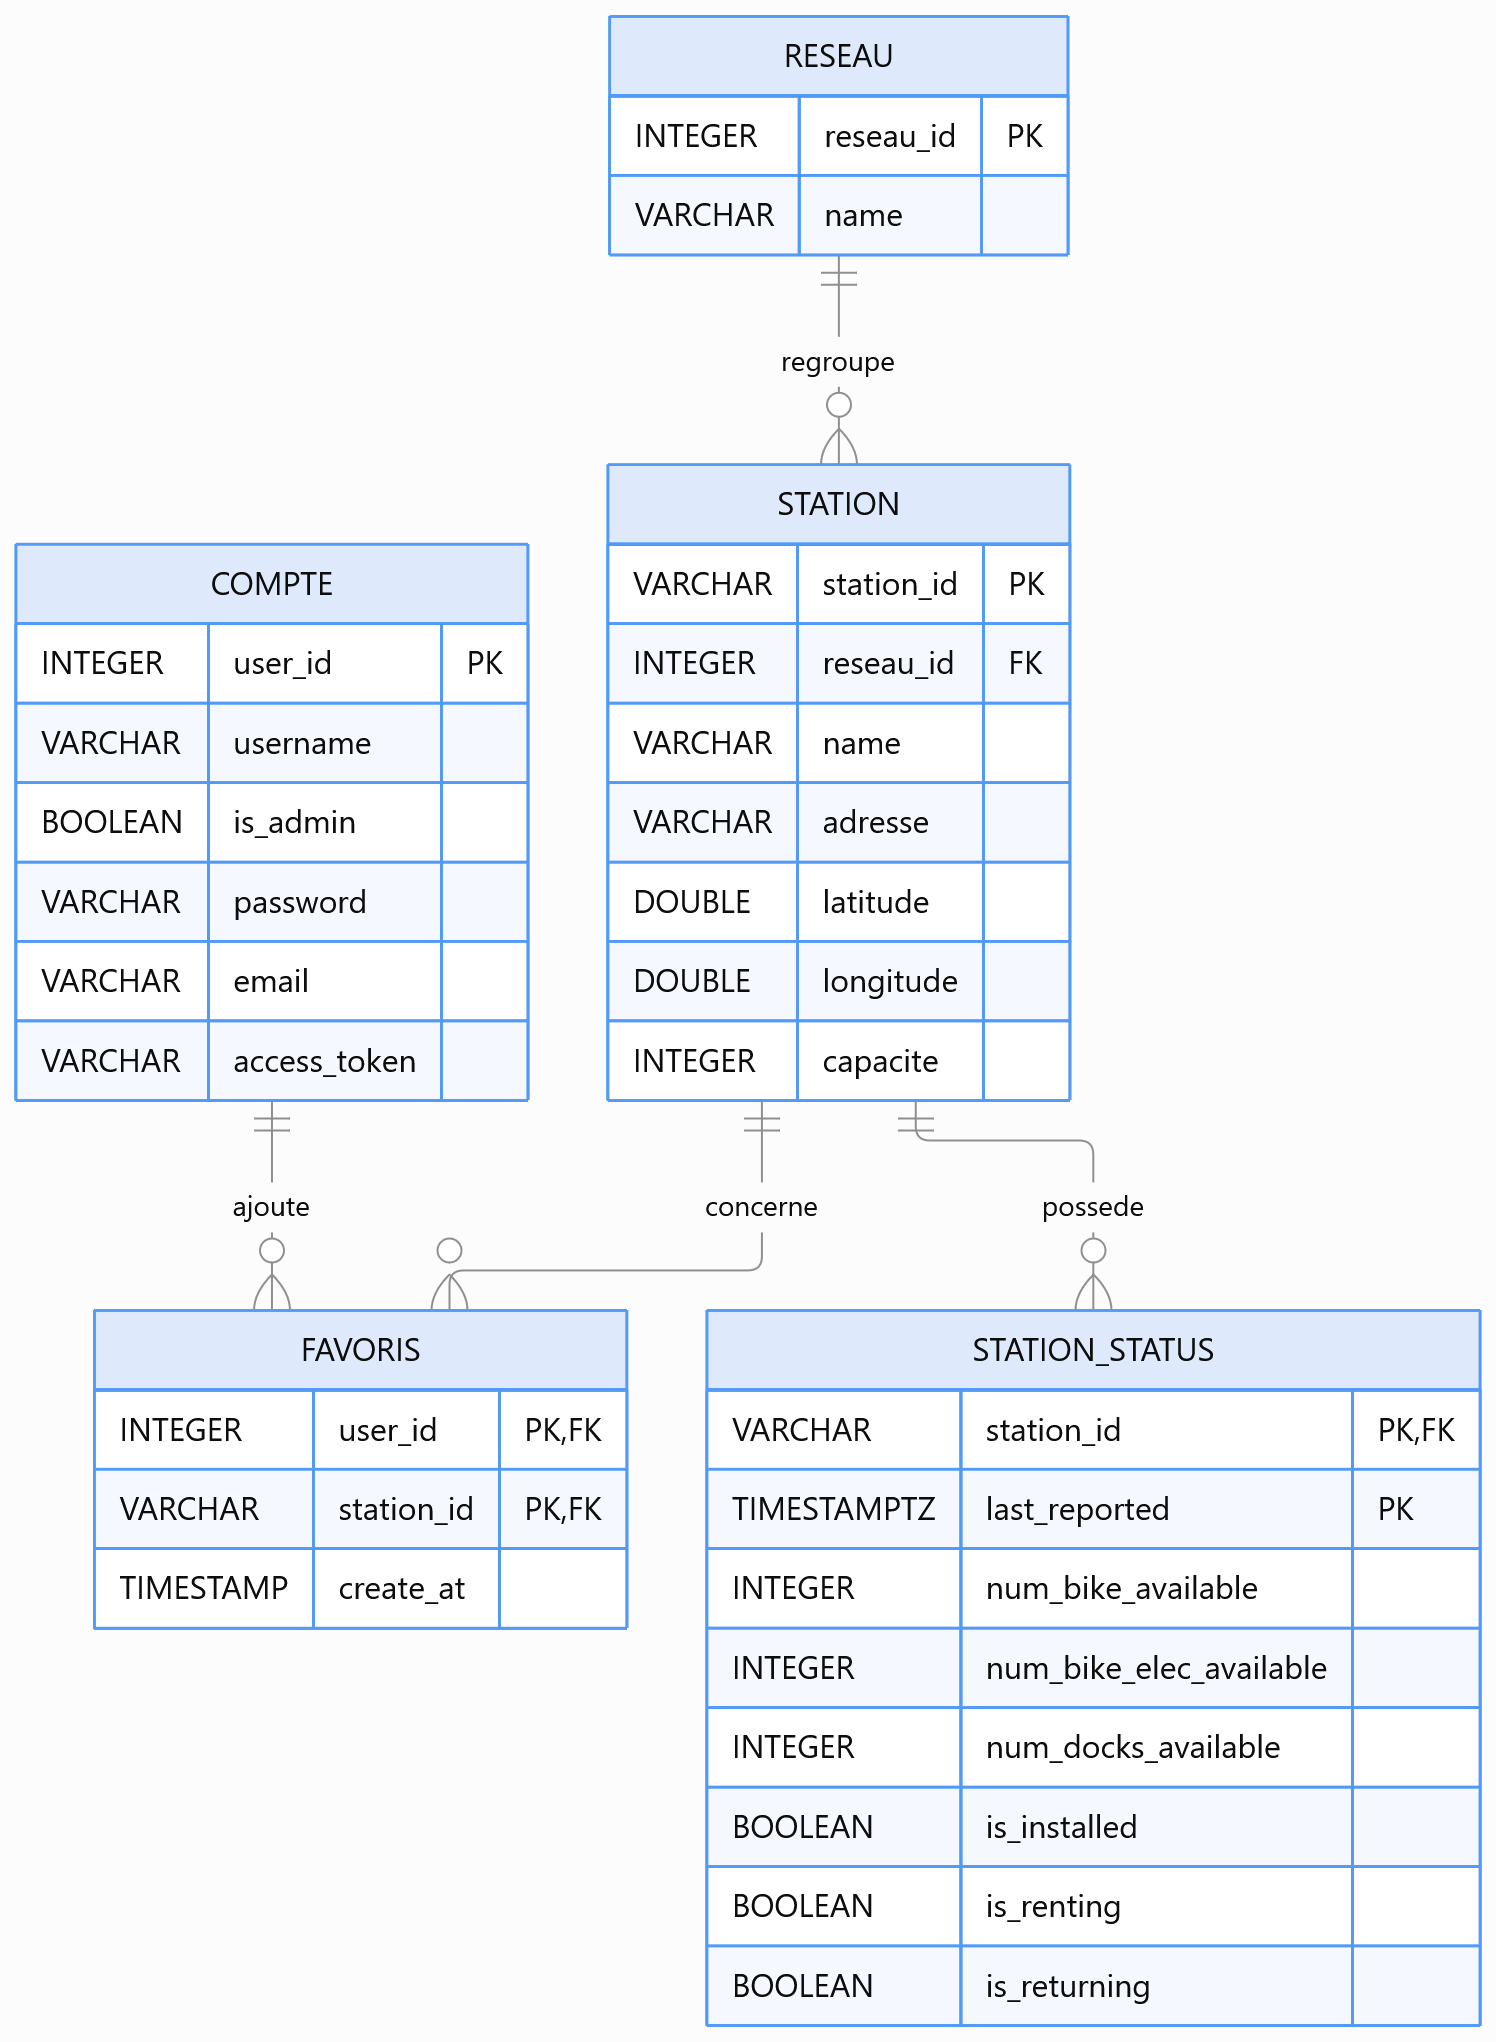
\includegraphics[keepaspectratio,alt={Modèle de données}]{../ressources/Diagramme/modele_BDD.png}}
Pour l'instant, notre réseau n'est composé que de celui de Bordeaux (id
1), mais il est possible d'ajouter d'autres villes.

Il est à noter que certaines difficultés ont été rencontrées en
confrontant notre application aux données réelles de Bordeaux sur
plusieurs semaines. Parmi ces dernières, nous avons identifié plusieurs
particularités nécessitant un nettoyage préalable :

\begin{itemize}
\item
  Stations en maintenance ou hors service : Certains relevés indiquent
  une station comme ouverte (is\_renting = true), alors que la somme des
  vélos disponibles et des places libres est strictement inférieure à la
  capacité officielle de la station (bornes défectueuses ou vélos
  bloqués).
\item
  Données figées ou absences de réponse : Il arrive ponctuellement que
  l'API de la ville renvoie des données obsolètes (horodatage
  last\_reported inchangé pendant plusieurs heures) ou subisse une
  micro-coupure réseau.
\end{itemize}

Notre module de collecte a été conçu pour filtrer les doublons temporels
et ignorer les relevés incohérents afin de ne pas fausser nos calculs
statistiques. Ce pré-traitement est notamment effectué au sein du DAO
des stations.

Le rôle de Véloscope de s'arrête pas à la simple extraction de ces
données. À partir de ces relevés bruts archivés toutes les 1h, VeloScope
produit ses propres indicateurs à forte valeur ajoutée. L'application
apporte à l'utilisateur des informations quant à l'état d'une station à
chaque instant, calcule des pourcentages de temps passé en pénurie ou en
saturation, la durée moyenne de ces épisodes d'indisponibilité, un score
global de fiabilité sur 100, ainsi qu'un score de recommandation
personnalisé. Ces calculs ne sont pas stockés dans notre base de données
mais effectués à la volée.

\pagebreak

\section{Architecture et système de
stockage}\label{architecture-et-systuxe8me-de-stockage}

\subsection{Nature de l'application et choix
technologiques}\label{nature-de-lapplication-et-choix-technologiques}

Notre objectif principal était de créer une application fiable et facile
à faire évoluer. Ainsi, nous avons fait le choix d'utiliser les outils
suivants et de la découper en plusieurs briques.

Pour ce faire, nous avons utilisé les outils technologiques suivants.
Notre projet utilise entièrement le langage de programmation Python
connu pour sa clarté et sa puissance quant à l'analyse de données. Nous
avons choisi FastAPI pour gérer la partie invisible de l'application.
Elle réalise les calculs, gère la sécurité et communique avec la base de
données. ELle est connue pour être rapide et génère automatiquement une
documentation claire de toutes ses commandes. Notre base de données est
stockée grace au logiciel spécialisé PostgreSQL. Il est sécurisé et
permet le stockage d'une grande quantité d'informations. Ainsi, il
conserve l'historique des relevés des stations vélo de Bordeaux. Enfin,
l'utilisateur intéragit avec notre application dans son navigateyr via
une interface visuelle grâce à l'outil Streamlit.

\subsection{Schéma d'architecture et décomposition en
couche}\label{schuxe9ma-darchitecture-et-duxe9composition-en-couche}

Comme évoqué précédemment notre code est organisé en cinq couches qui
communiquent entre elles de manière ordonnée. Cette structure est
schématisée par la diagramme d'architecture. L'application est articulée
autour du Backend qui contient la logique de gestion des données, et du
Frontend qui permet à l'utilisateur d'intéragir avec l'application.
L'application communique également avec une source de données externe
afin de récupérer les informations sur des stations de vélo.

\begin{figure}[H]

{\centering \pandocbounded{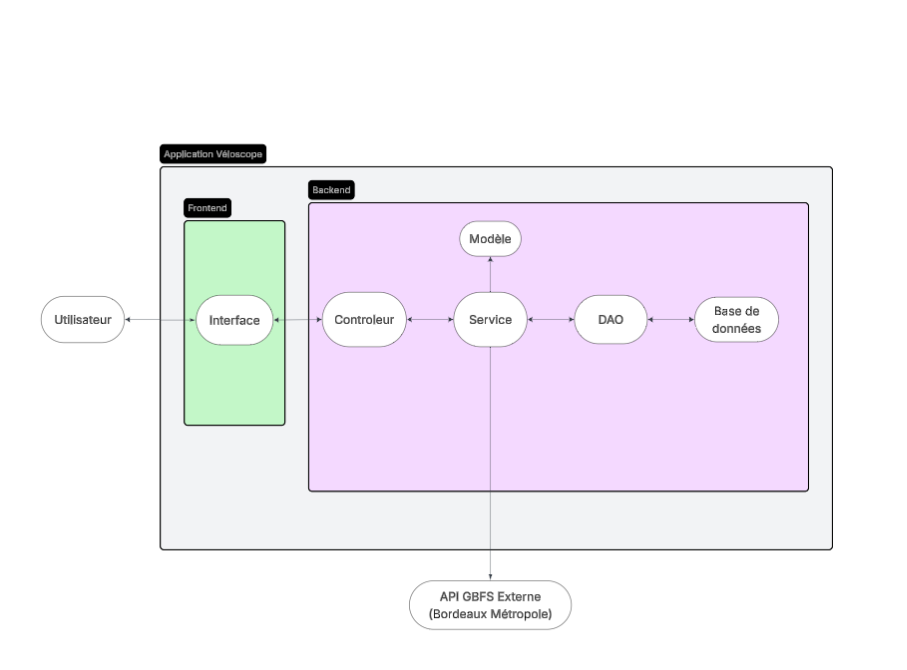
\includegraphics[keepaspectratio]{../ressources/Diagramme/diagramme_architecture_final.png}}

}

\caption{Diagramme d'architecture}

\end{figure}%

La première couche, la seule visible par l'utilisateur est l'Interface
(Streamlit). On l'appelle le Frontend. C'est la vitrine de notre
application. Elle affiche les différentes pages et permet à
l'utilisateur d'intéragir avec l'application. Elle ne fait aucun calcul
complexe elle même. Elle transmet seulement les instructions au Backend.

Les quatre autres couches forment le Backend.

La deuxième couche est celle des controleurs ( API FastAPI). C'est cette
couche qui reçoit les demandes de l'interface, verifient qu'elles soient
bien formulées et les transmets aux services.

Les services sont la troisième couche du code. C'est ici que de trouve
toute la logique métier de l'application. Cette partie rassemble
l'ensemble des méthodes qui permettent à notre application de
fonctionner (calcul du score de fiabilité, tri des recommandations,
vérification des mots de passe, etc). C'est également un Service qui va
chercher les données sur Internet auprès de l'API de la ville de
Bordeaux.

La quatrième couche du projet est les modèles. Ils permettent de
structurer les données utilisées par l'application. Ils définissent à
quoi ressemble une station ou un utilisateur dans notre code.

Enfin, la derniere couche est constituée des DAO. Les DAO (Data Access
Objects) assurent la communication avec la base de données. Ils peuvent
lire et écrire dans la base de données PostgreSQL.

\pagebreak

\section{Réponse aux besoins}\label{ruxe9ponse-aux-besoins}

\subsection{Détails de la fonctionnalité F5 : Recommandation de
station}\label{duxe9tails-de-la-fonctionnalituxe9-f5-recommandation-de-station}

Nous détaillons dans cette partie la fonctionnalité F5 : Recommandation
d'une station. Il s'agit de la fonctionnalité principale de notre
application. Un utilisateur peut ainsi fournir une adresse de Bordeaux,
par exemple ``Place Pey Berland'', choisir le nombre maximal de stations
qu'il veut avoir en recommandation et le périmètre de recherche (rayon
en km ayant pour centre l'adresse indiquée). L'application lui renvoit
les stations recommandées selon le meilleur compromis compte tenu de la
distance et de la fiabilité. Le diagramme de séquence de cette
fonctionnalité est proposé ci-contre.

\pandocbounded{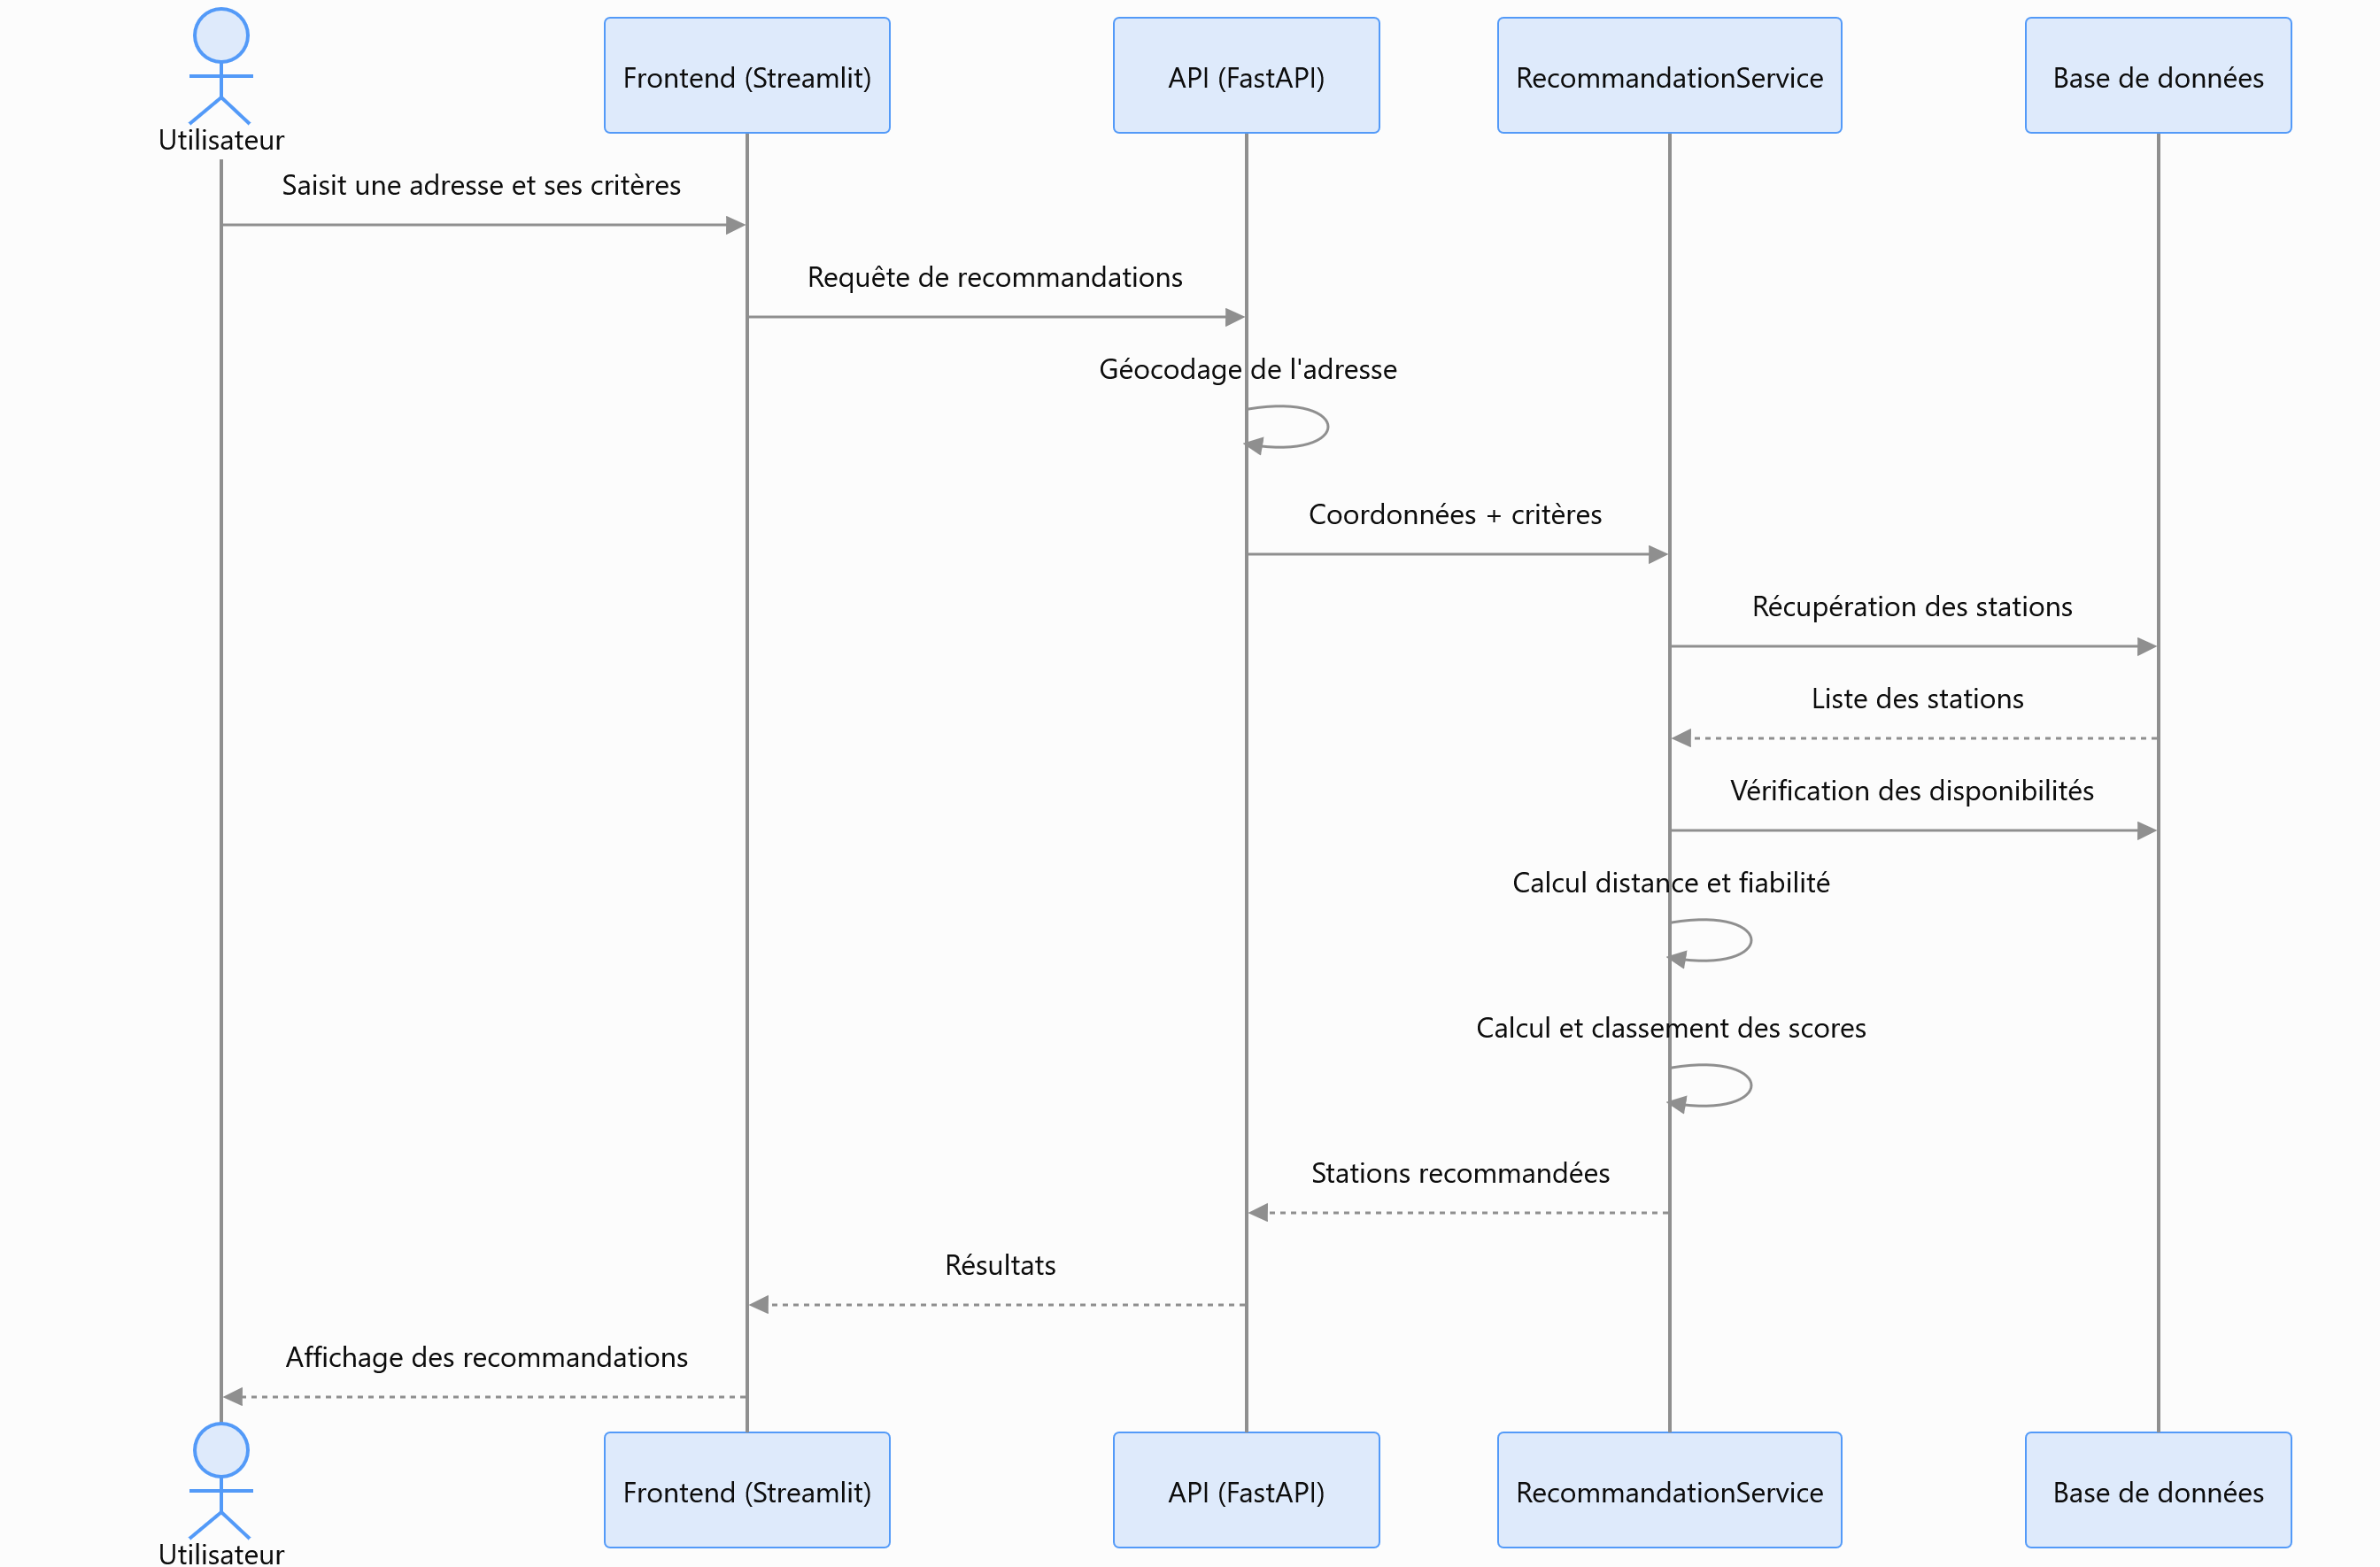
\includegraphics[keepaspectratio,alt={Diagramme de séquence F5}]{../ressources/Diagramme/diagramme_sequence_F5.png}}
Zoomons sur ce processus de manière plus précise.

\begin{enumerate}
\def\labelenumi{\arabic{enumi})}
\tightlist
\item
  Recherche à partir d'une adresse
\end{enumerate}

Partons de la page \texttt{recommendation}du frontend. Dans l'interface,
une zone de saisie est crée afin que l'usager saisisse une adresse à
Bordeaux et choisisse le nombre maximal de résultats ainsi qu'un rayon
de recherche. L'utilisateur clique sur le bouton ``Rechercher des
stations''. À ce moment, la requête HTTP est envoyée au backend sous
forme de dictionnaire.

\begin{figure}

\centering{

\pandocbounded{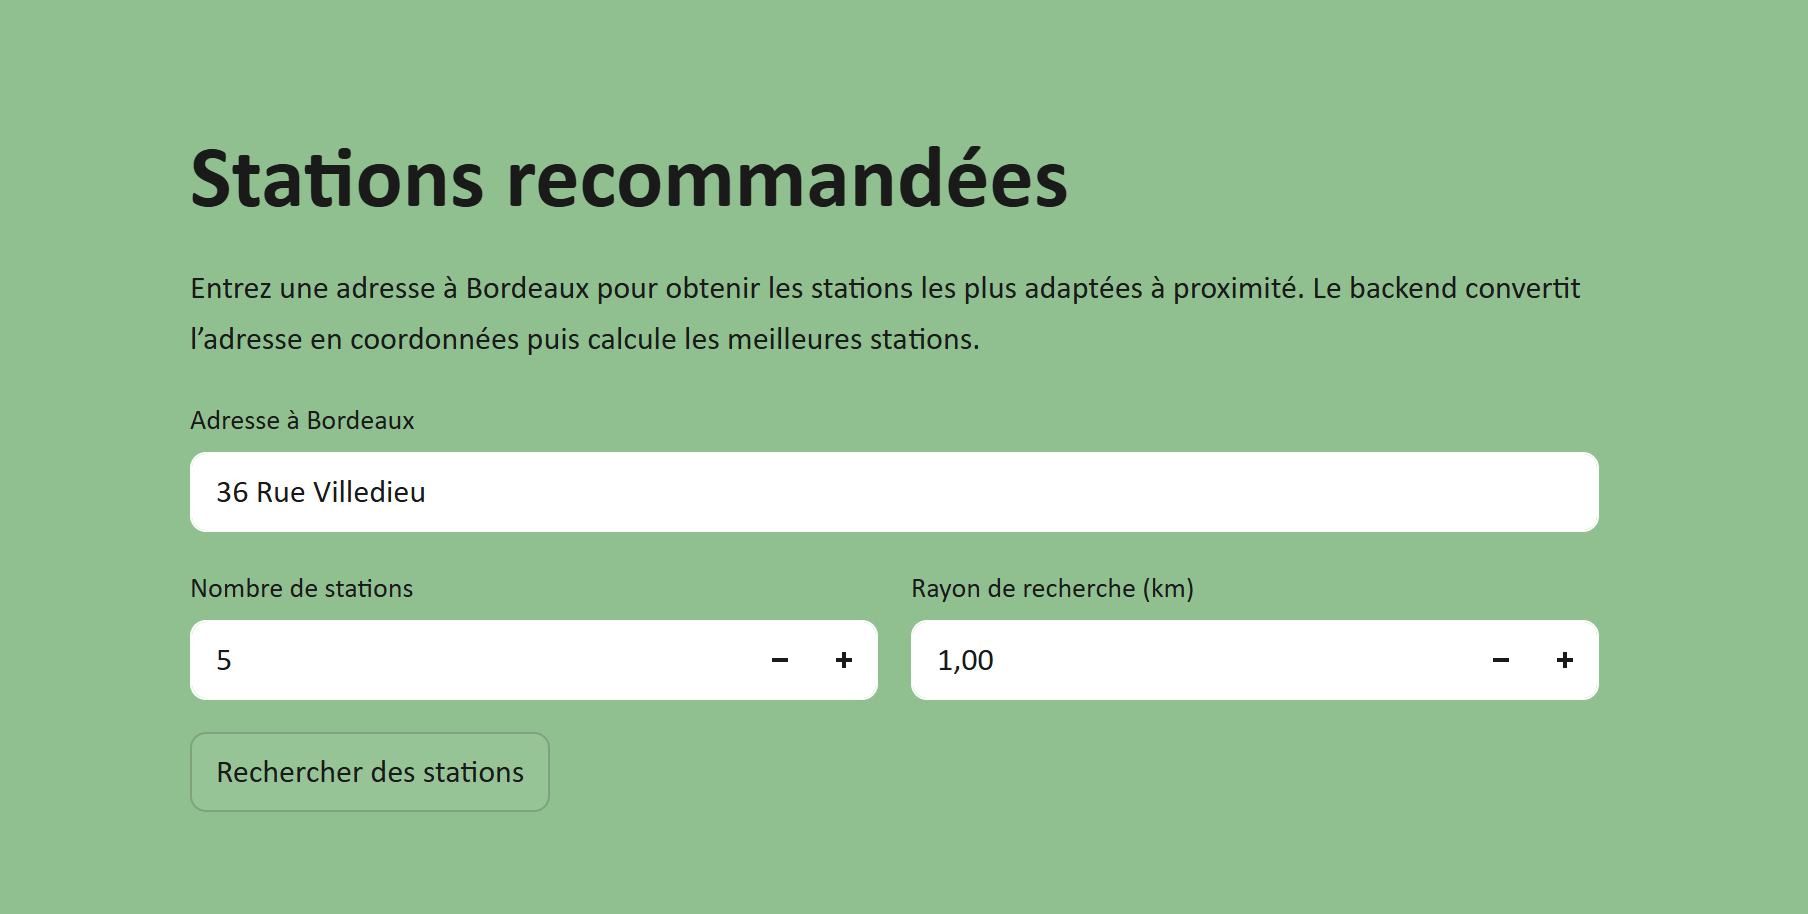
\includegraphics[keepaspectratio]{../ressources/Screenshots/reco_interface_requete.png}}

}

\caption{\label{fig-reco-form}Saisie de l'adresse et des critères de
recherche dans l'interface.}

\end{figure}%

\begin{enumerate}
\def\labelenumi{\arabic{enumi})}
\setcounter{enumi}{1}
\tightlist
\item
  Traitement de la requête : conversion de l'adresse
\end{enumerate}

Le routeur FastAPI dans le controller \texttt{recommendation} reçoit
cette requête. Cette fonction se charge de vérifier que l'on dispose
d'une position, puis délègue le travail au service de recommandation.
Pour vérifier que l'utilisateur a transmis une position avec son adresse
et la convertir en coordonnées, on utilise le géocodage.

Pour ce faire, le controller appelle la fonction
\emph{geocode\_bordeaux\_address} dans utils. Cette fonction interroge
\textbf{Nominatim}, le service de géocodage d'OpenStreetMap, grâce au
package python \texttt{requests}. Il ajoute « Bordeaux, France » à
l'adresse saisie, demande un résultat au format JSON et fixe un délai
maximal de réponse de dix secondes. Les coordonnées retournées sont
ensuite vérifiées : elles doivent se situer dans une zone géographique
approximative autour de Bordeaux. Ce contrôle permet de rejeter les
résultats manifestement éloignés, sans correspondre exactement aux
limites administratives de la métropole. Une exception HTTP est levée en
cas d'erreur.

L'API peut également recevoir directement une latitude et une longitude,
sans passer par le géocodage (mais cela n'est pas disponible sur
l'interface Streamlit). Dans les deux cas, le service de recommandation
travaille finalement à partir de coordonnées.

\begin{enumerate}
\def\labelenumi{\arabic{enumi})}
\setcounter{enumi}{2}
\tightlist
\item
  Sélection des stations et calcul du score
\end{enumerate}

Le service récupère la liste de toutes les stations par appel au DAO et
calcule la distance à vol d'oiseau entre la position recherchée et
chaque station. Il utilise ensuite le dernier statut enregistré pour
écarter les stations qui ne sont pas installées, qui ne permettent pas
l'emprunt ou qui ne disposent d'aucun vélo, comme elles ne constituent
pas une bonne recommandation. Pour les stations qui ne sont pas
écartées, on calcule le score de fiabilité global par appel au service
\texttt{fiabilite}.

Le paramètre \texttt{rayon\_km} permet de limiter la recherche aux
stations situées dans un rayon donné. Il est facultatif dans l'API :
sans ce paramètre, aucune distance maximale n'est appliquée. Le
paramètre \texttt{limite}, égal à 5 par défaut, détermine le nombre
maximal de résultats renvoyés. Dans l'interface, l'usager peut choisir
de 1 à 10 stations et un rayon de 0,1 à 10 km ; le rayon proposé par
défaut est de 1 km.

Les stations qui satisfont ces critères sont classées selon un score
combinant à parts égales la proximité et la fiabilité :

{[} S\_\{\mathrm{recommandation}\} = 0\{,\}5
\times S\_\{\mathrm{proximité}\} + 0\{,\}5
\times S\_\{\mathrm{fiabilité}\} {]}

Le score de proximité décroît avec la distance selon une fonction
gaussienne :

{[} S\_\{\mathrm{proximité}\} =
e\textsuperscript{\{-\textbackslash frac\{d}2\}\{2\sigma\^{}2\}\},
\qquad \sigma = 1~\mathrm{km} {]}

où d désigne la distance entre l'adresse recherchée et la station. Le
score de fiabilité est calculé à partir de l'état actuel de la station
et de son historique : les proportions de temps passé vide ou saturée
ainsi que la durée moyenne des épisodes correspondants. Il est renvoyé
sous la forme d'une valeur comprise entre 0 et 1.

La décroissance gaussienne favorise nettement les stations proches, tout
en évitant une coupure brutale au-delà d'une distance fixée. Avec
(\sigma = 1) km, une station située à 1 km conserve un score de
proximité d'environ 0,61, mais celui-ci baisse rapidement plus loin.
Cela est pratique pour l'usager : la distance compte, sans être le seul
critère, car la fiabilité peut départager des stations proches.

Une fois le calcul de chaque score effectué et le classement établit,
l'API renvoie au frontend au plus le nombre de stations demandé. Si deux
scores de recommandations sont égaux, on classe par distance, puis par
ordre alphabétique. Pour chaque station, la réponse contient ses
informations, la distance arrondie au millième de kilomètre, le score de
fiabilité et le score de recommandation arrondi à quatre décimales.

\begin{enumerate}
\def\labelenumi{\arabic{enumi})}
\setcounter{enumi}{3}
\tightlist
\item
  Résultats affichés et vérification de l'API
\end{enumerate}

L'interface présente les stations recommandées avec leur nom, leur
adresse, leur distance et leurs scores. La distance est une distance à
vol d'oiseau : elle ne représente pas un trajet réel à vélo par le
réseau de rues.

\begin{figure}

\centering{

\pandocbounded{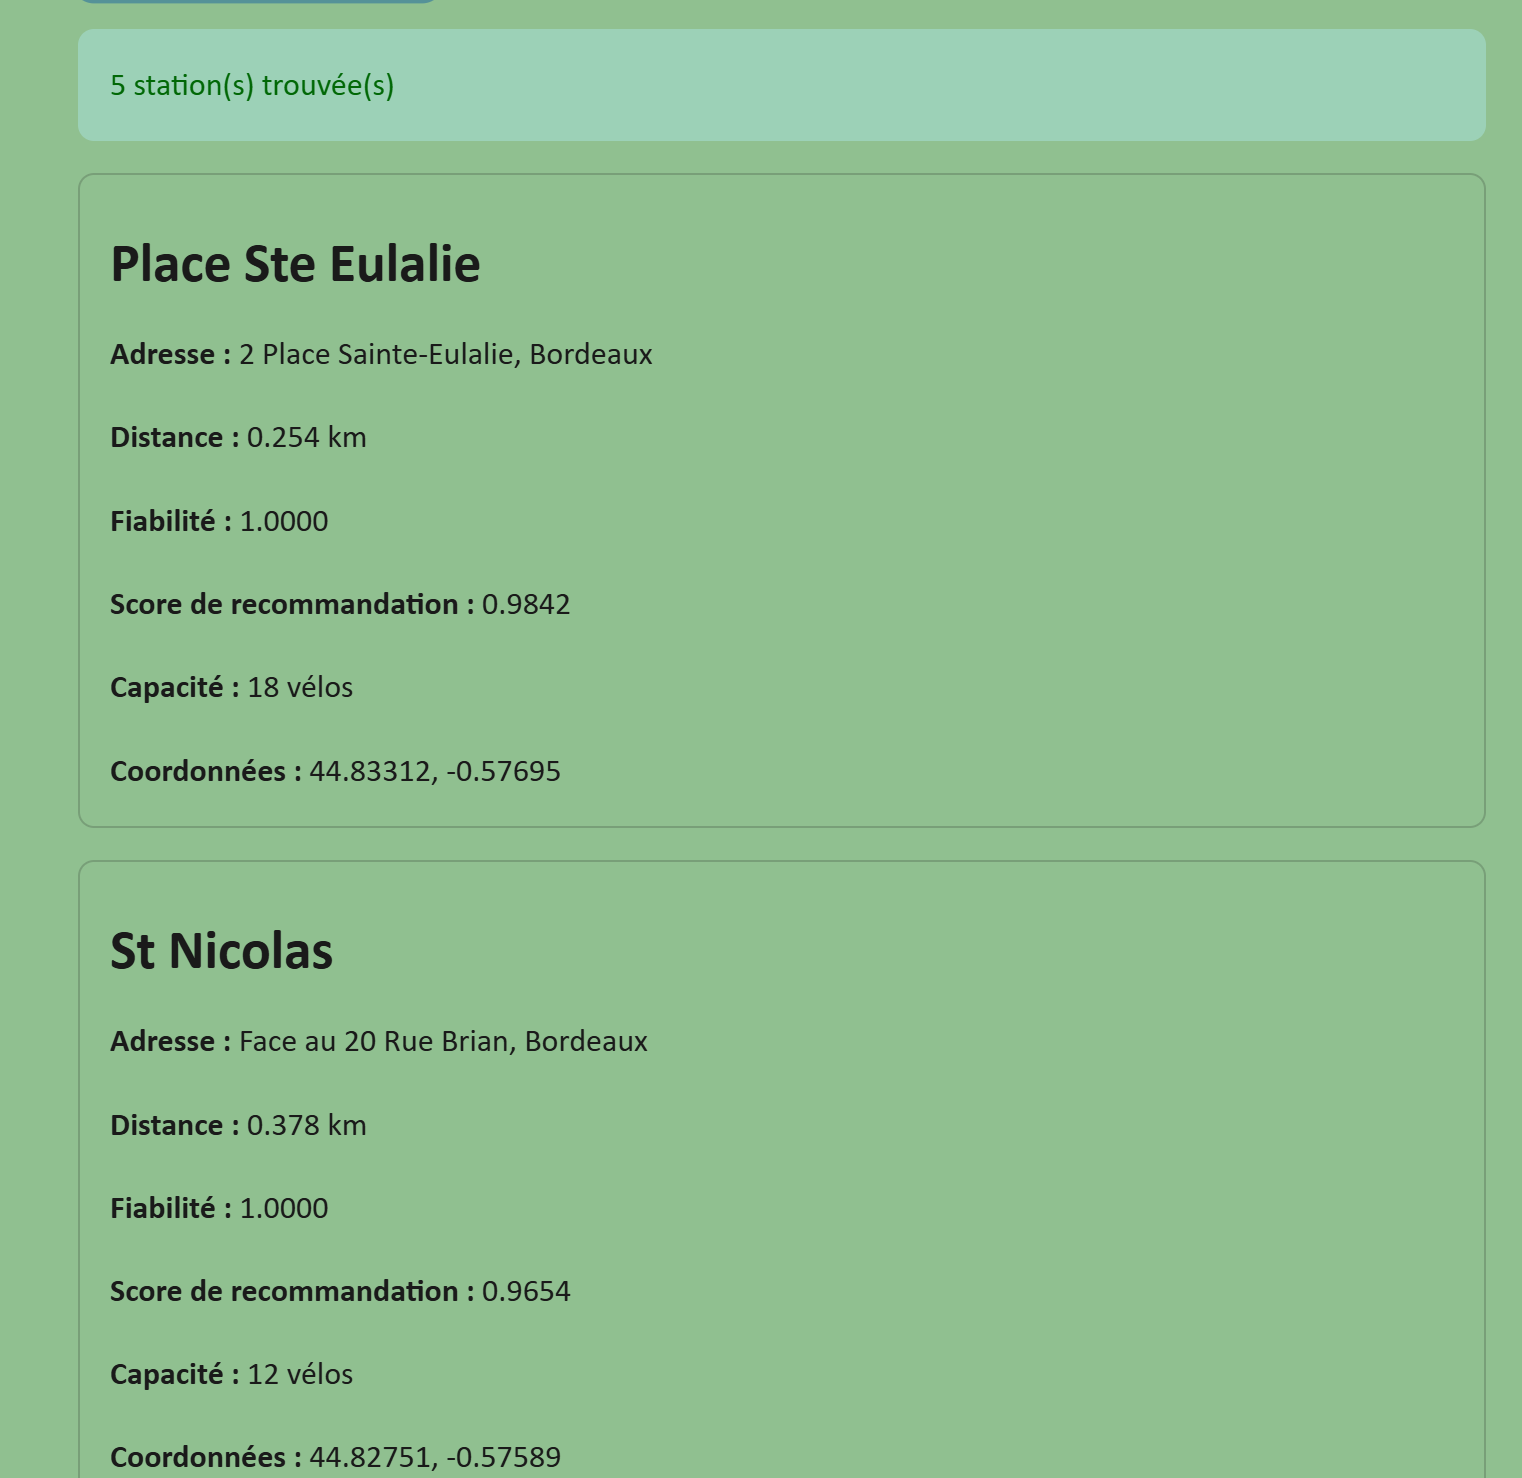
\includegraphics[keepaspectratio]{../ressources/Screenshots/reco_interface_resultats.png}}

}

\caption{\label{fig-reco-resultats}Stations recommandées affichées dans
l'interface.}

\end{figure}%

L'endpoint \texttt{GET\ /recommendation/} est également documenté dans
Swagger. Sa documentation permet de vérifier les paramètres acceptés ---
adresse ou coordonnées, limite et rayon --- et la structure de la
réponse renvoyée.

\begin{figure}

\centering{

\pandocbounded{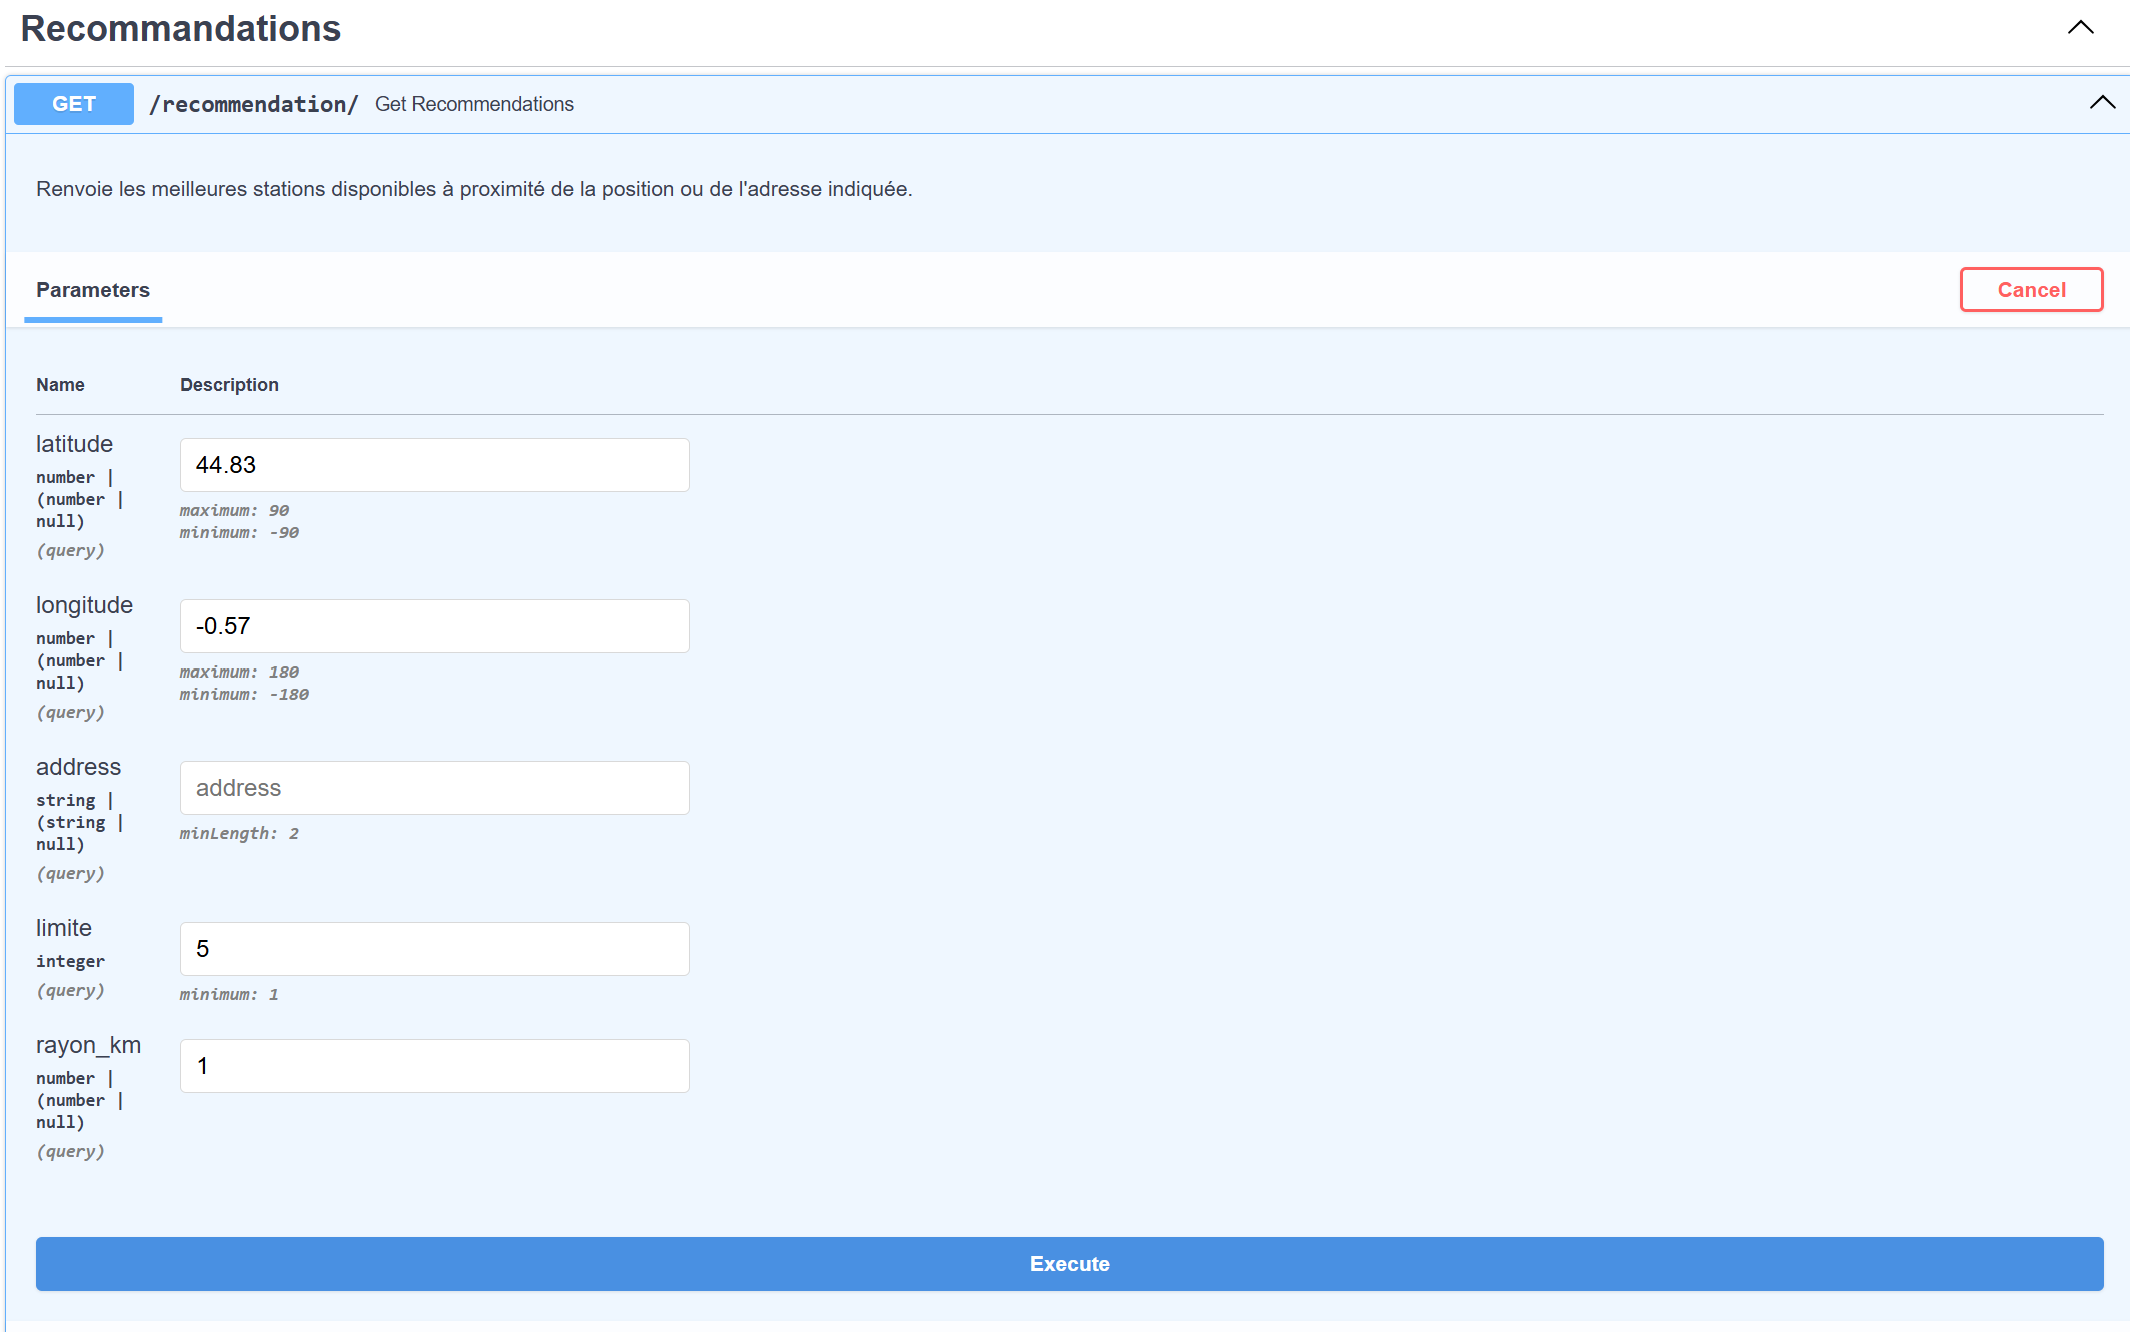
\includegraphics[keepaspectratio]{../ressources/Screenshots/reco_swagger_requete.png}}

}

\caption{\label{fig-reco-swagger-requete}Requête de recommandation et
paramètres dans Swagger.}

\end{figure}%

\begin{figure}

\centering{

\pandocbounded{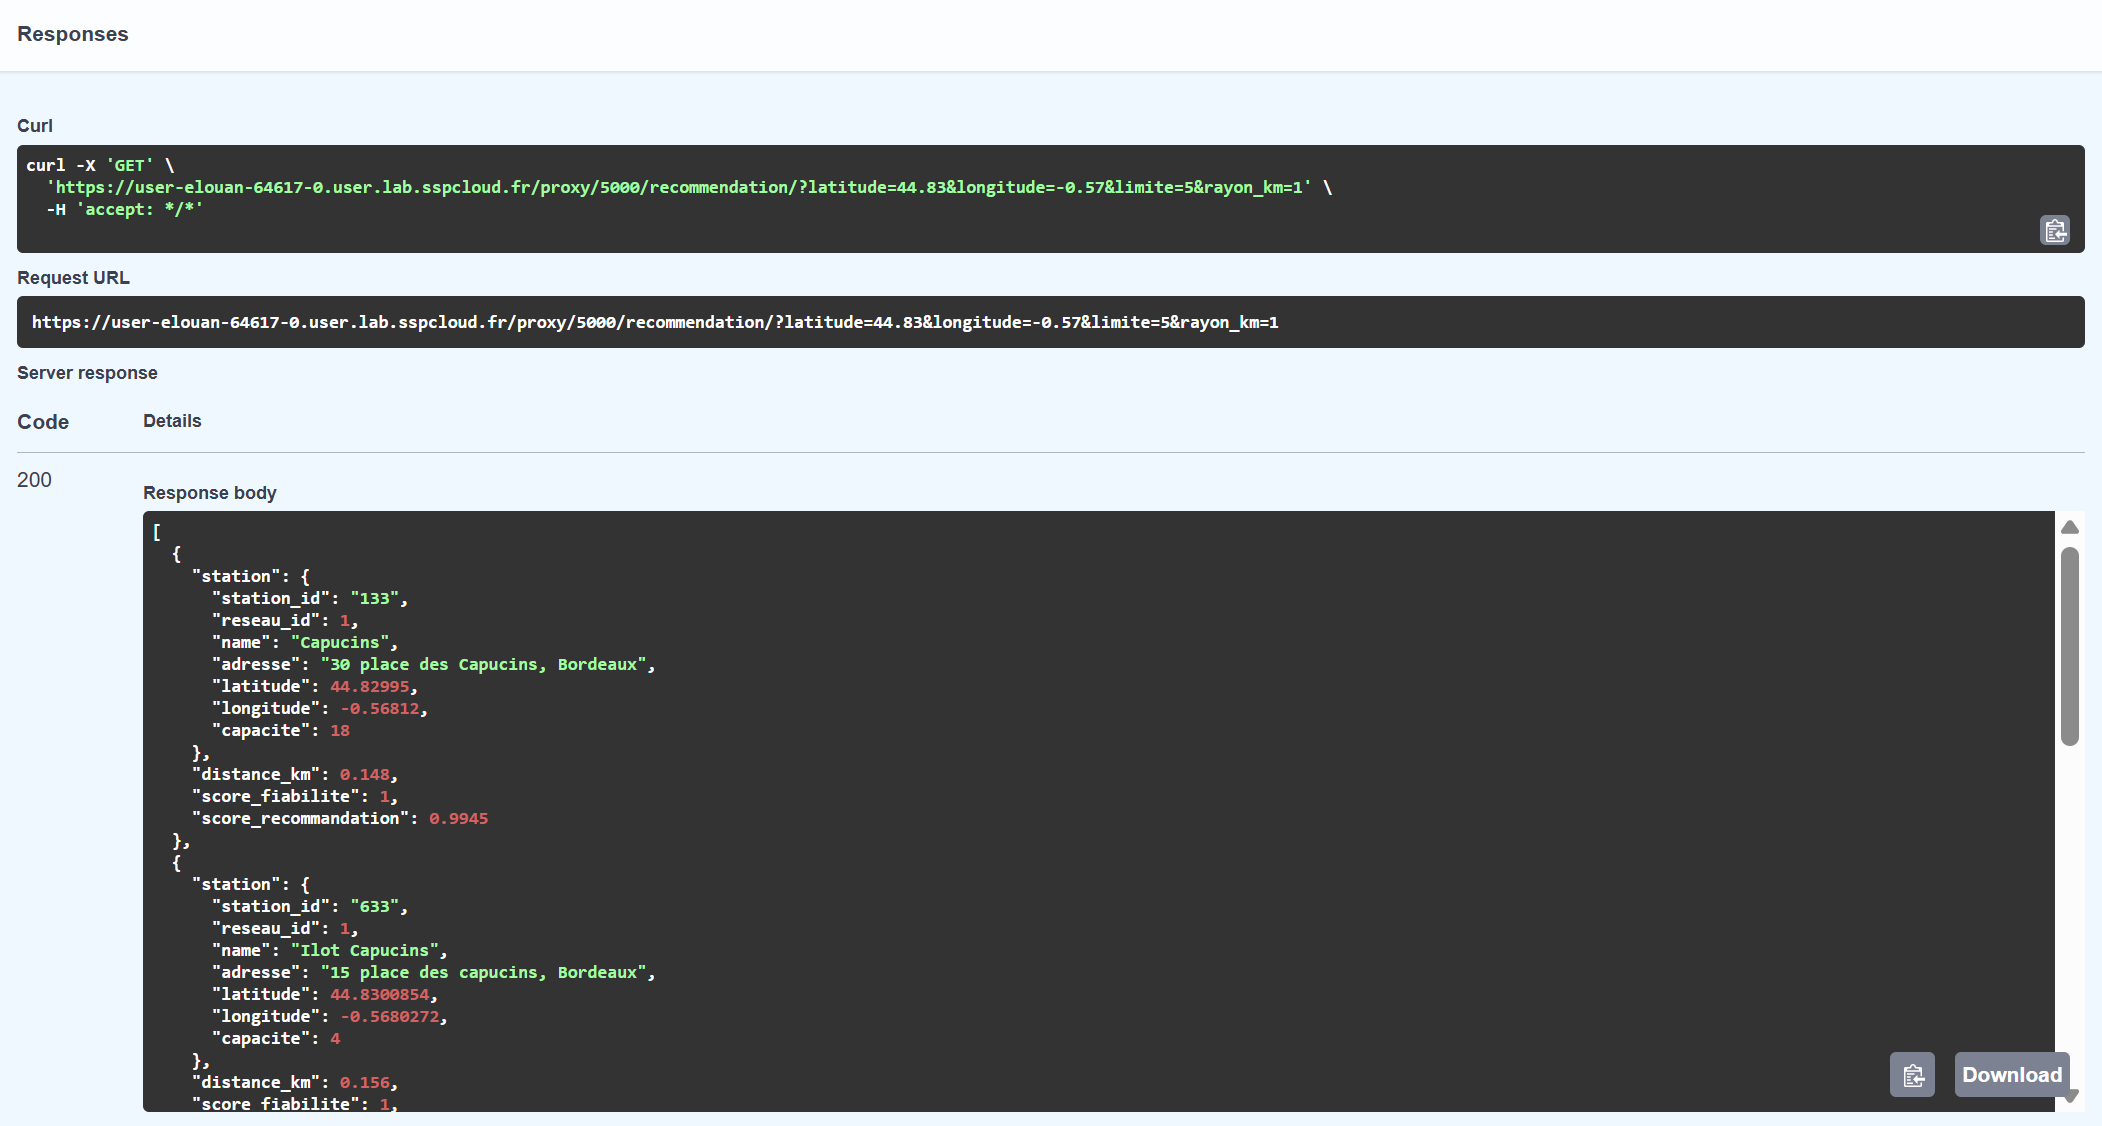
\includegraphics[keepaspectratio]{../ressources/Screenshots/reco_swagger_reponse.png}}

}

\caption{\label{fig-reco-swagger-reponse}Exemple de réponse renvoyée par
l'API dans Swagger.}

\end{figure}%

Les tests existants vérifient notamment l'appel de l'API avec des
coordonnées, la prise en charge d'une adresse à l'aide d'un géocodeur
simulé et le rejet de coordonnées hors limites. Le fonctionnement
complet du classement --- filtres, calcul des scores et tri --- pourrait
être davantage couvert par des tests. La recherche par adresse dépend
aussi de la disponibilité de Nominatim et de la qualité de l'adresse
saisie.

\subsection{Synthèse des autres
fonctionnalités}\label{synthuxe8se-des-autres-fonctionnalituxe9s}

\subsubsection{Compte et authentification
(F1)}\label{compte-et-authentification-f1}

Toute utilisation de l'application nécessite un compte. Le visiteur peut
en créer un via un formulaire renseignant un nom d'utilisateur (30
caractères maximum), une adresse mail et un mot de passe à confirmer. Si
le nom est déjà utilisé, l'API renvoie une erreur 400. Les comptes créés
sont non-administrateurs par défaut, seuls les administrateurs pouvant
attribuer ces droits.

Pour sécuriser les mots de passe, ceux-ci ne sont jamais stockés en
clair, mais hachés via SHA-256, en combinaison avec l'identifiant de
l'utilisateur. Une fois le compte créé, le visiteur est invité à se
connecter. Le service compare alors l'empreinte du mot de passe saisi à
celle stockée en base. En cas de succès, un jeton aléatoire est généré,
enregistré sur le compte et renvoyé avec les informations de
l'utilisateur ; chaque connexion remplace le jeton précédent. En cas
d'identifiants invalides, l'API renvoie une erreur 401. Les routes
protégées (stations, favoris, modification et suppression de compte)
nécessitent également un jeton valide. De même, les pages de
recommandation, de recherche d'itinéraire et de gestion des utilisateurs
vérifient sa présence en session et affichent un message d'erreur en son
absence.

\subsubsection{Favoris (F1)}\label{favoris-f1}

Un utilisateur peut consulter ses stations favorites depuis l'onglet
\textbf{favoris}. Il peut choisir de supprimer un favoris depuis cette
page par une requête HTTP. Une station peut être ajoutée en favoris
depuis la page de liste déroulante contenant toutes les stations du
réseau, ou depuis la page de recherche d'une station à partir de son
nom. Une station déjà présente dans les favoris renvoie une erreur 409.

\subsubsection{Collecte des données depuis l'API externe
(F2)}\label{collecte-des-donnuxe9es-depuis-lapi-externe-f2}

L'insertion des données externes, récupérées auprès de l'API Le Vélo,
dans notre base de données repose sur une séparation entre la collecte
des données brutes et leur adaptation au format attendu, afin de
faciliter l'évolution du système en cas de modification du format des
données sources. Le fichier \texttt{background\_collection} organise la
collecte périodique et son lancement en arrière-plan. Lors du démarrage
du backend, il est possible d'activer ou non ce dispositif.

Si la collecte est activée, elle est réalisée de manière périodique et
en arrière-plan, afin de ne pas bloquer le fonctionnement principal de
l'API. Le service \texttt{Collection} est alors sollicité. Il s'appuie
sur un \emph{provider}, qui coordonne la collecte et l'adaptation des
données. Celui-ci repose sur deux composants : un \texttt{GBFSClient},
chargé de récupérer les données brutes depuis l'API externe via des
requêtes HTTP (\texttt{requests}), et un adaptateur (\emph{Adapter}),
chargé de convertir le JSON reçu en objets métier. Le service de
collecte transmet ensuite ces objets au DAO, qui se charge de leur
insertion en base de données.

\subsubsection{Consultation de station
(F3)}\label{consultation-de-station-f3}

L'utilisateur peut aussi utiliser la page ``Consultation d'une station''
pour se renseigner sur une station précise. Il doit saisir le nom de la
station, puis la sélectionne parmi la liste qui s'affiche. Il obtient
alors :

\begin{itemize}
\item
  Son identifiant, adresse, coordonnées ainsi que des informations sur
  son état actuel (si la station est disponible, vide, saturée, non
  opérationnelle ou inconnue, le nombre de vélos qui y sont disponibles
  dont les vélos électriques, le nombre de places disponibles, sa
  capacité, son taux de remplissage ainsi que la date et le détail de
  son dernier relevé),
\item
  L'évolution de sa disponibilité sur 24h, 7 jours ou 31 jours; ainsi
  que les détails de sa fiabilité (son score actuel, la part du temps
  passée vide et saturée, la durée moyenne des épisodes de vide et de
  saturation, et l'évolution du score).
\end{itemize}

Une station est considérée comme disponible si elle est installée,
permet les emprunts et retours et possède au moins une place libre et un
vélo. Elle est renvoyé sous forme d'un booléen (1 si pisponible, 0
sinon). Le calcul de disponibilité est gérée par le service station.

\subsubsection{Fiabilité des stations
(F4)}\label{fiabilituxe9-des-stations-f4}

Comme indiqué plus haut, le score de fiabilité d'une station est calculé
à partir de l'historique de ses statuts selon la moyenne de 5
composantes : le pourcentage de temps passé vide et saturée, la durée
moyenne des périodes de vide et de saturation, et l'état actuelle de la
station (si elle est à la fois ni vide ni saturée). Il est à prendre
avec parcimonie : une station qui est toujours vide mais jamais saturée
possède un score non nul. Pour cette raison, on affiche de détail de
chaque composante qui a permis le calcul de la fiabilité afin de donner
davantage d'informations à l'utilisateur.

Le calcul du score se fait à partir du service fiabilité. Il est calculé
depuis la date la plus ancienne d'historique présent sur la base de
données. Le calcul de l'historique demandant de parcourir chaque date de
relevé présent sur la base de données en tenant compte des précédents,
il a été optimisé pour réutiliser les indicateurs ayant été déjà
calculés par le passé afin de ne pas les recalculer et éviter une
surcharge. La sélection des statuts qui ne concernent qu'une station
selon une date limite de début de relevé se fait grâce à une fonction de
la dao des status.

\subsubsection{Fonctionnalité
supplémentaire}\label{fonctionnalituxe9-suppluxe9mentaire}

L'utilisateur peut afficher la carte des stations du réseau. En
survolant les marqueurs des stations avec sa souris, l'utilisateur peut
en afficher le nom, l'adresse et la capacité.

\pagebreak

\section{Tests et qualité
logicielle}\label{tests-et-qualituxe9-logicielle}

Pour garantir que VeloScope produise des résultats fiables et résiste
aux erreurs d'utilisation comme aux aléas des données réelles de
Bordeaux, nous avons mené des vérifications structurées sur l'ensemble
des couches de l'application (interface Streamlit, API FastAPI, logique
métier, accès aux données et collecte). L'objectif était double :
vérifier que chaque fonctionnalité répond bien au cahier des charges
dans son fonctionnement normal, et s'assurer que l'application gère
proprement les situations dégradées, les saisies inattendues et les
imperfections des flux de données.Ces vérifications reposent à la fois
sur des tests automatisés, exécutés à chaque push par une chaîne
d'intégration continue, et sur des contrôles manuels.

\subsection{Vérification des fonctionnalités et des cas
limites}\label{vuxe9rification-des-fonctionnalituxe9s-et-des-cas-limites}

Nous avons testé le comportement de l'application aussi bien dans les
cas nominaux que dans des situations dégradées ou aux limites, afin
d'éviter les blocages, les calculs faussés ou les erreurs non maîtrisées
:

\textbf{Authentification, droits et gestion des favoris (F1) :} Nous
avons vérifié qu'un compte ne peut être créé que lorsqu'il respecte les
modalités suivantes. L'utilisateur doit impérativement confirmer son mot
de passe, la longueur de son nom d'utilisateur est contrôlé, et si ce
nom est déjà pris, le compte est rejeté. Nous avons également testé le
hachage des mots de passe, la génération puis le remplacement du token à
chaque nouvelle connexion, ainsi que le contrôle d'accès via token.
L'accès est effectivement refusé lorsqu'un token est absent ou invalide.
Le blocage des routes d'administration pour un compte standard a
également été vérifié. Nous avons également contrôlé l'ajout, la
consultation et la suppression des stations favorites, y compris lorsque
l'utilisateur tente d'ajouter une station déjà enregistrée ou
inexistante.

\begin{itemize}
\item
  \textbf{Collecte et nettoyage des données (F2) :} Nous avons contrôlé
  la récupération périodique des flux GBFS de Bordeaux Métropole et
  l'archivage des relevés dans PostgreSQL sans écraser l'historique
  existant. Cela permet de pouvoir reconstituer l'état passé du réseau.
  Nous avons prêté une attention particulière aux anomalies observées
  sur les données réelles : doublons temporels, horodatages figés sur
  plusieurs relevés consécutifs ou incohérences entre la capacité
  déclarée et les vélos ou places libres disponibles, afin que ces cas
  ne faussent pas les analyses ultérieures.
\item
  \textbf{Consultation, fiabilité et recommandation (F3, F4, F5) :} Nous
  avons testé la recherche de stations (à partir de 3 caractères
  saisis), l'affichage des états et des disponibilités ainsi que les
  courbes d'évolution sur les différentes fenêtres temporelles (24
  heures, 7 jours, 30 jours). Nous avons également vérifié le calcul des
  indicateurs de vide et de saturation ainsi que le score de fiabilité
  sur des jeux de données variés (station régulière, station souvent
  vide ou saturée, historique court ou incomplet), et testé le moteur de
  recommandation dans plusieurs configurations : adresse hors de
  l'agglomération bordelaise ou introuvable, rayon de recherche étroit
  ou sans station utilisable, et classement selon le score combinant
  proximité et fiabilité.
\item
  \textbf{Parcours utilisateur sur l'interface Streamlit :} Nous avons
  contrôlé la cohérence des informations affichées entre les différentes
  pages, la lisibilité des graphiques et de la carte, ainsi que la
  présence de messages d'erreur clairs et compréhensibles lorsqu'aucune
  donnée ne correspond à la demande ou qu'un accès nécessite une
  authentification.
\end{itemize}

\subsection{Tests automatisés}\label{tests-automatisuxe9s}

Parallèlement à l'écriture du code, nous avons développé des tests avec
pytest, qui suivent l'architecture en couches décrite en section 3 : les
services, les contrôleurs et les DAO disposent chacun de leurs tests
(dossiers tests/test\_service, tests/test\_controller et
tests/test\_dao), soit plus de 150 cas de test. Chaque scénario est
structuré selon la convention GIVEN / WHEN / THEN : état initial, action
testée, résultat attendu.

Le principe est de tester chaque couche isolément, en remplaçant les
couches voisines par des objets simulés (unittest.mock). Les tests sont
ainsi rapides (quelques secondes pour l'ensemble des tests unitaires),
déterministes et indépendants du réseau comme de l'API de la métropole.

Dans la couche Service nous testons principalement: la création de
compte et la connexion, la recherche de station, le taux de remplissage,
l'historique sur 24 h / 7 j / 30 j, le calcul du score de fiabilité
(durées et pourcentages de vide et de saturation, évolution, cas sans
historique), les favoris. Pour ce faire, nous remplaçons les DAO par des
MagicMock.

Dans la couche contrôleurs nous testons principalement: les routes
FastAPI : codes HTTP (200, 400, 401, 403, 404, 422, 500), la validation
des paramètres, les droits administrateur, les tokens , le cloisonnement
des favoris par utilisateur.

Dans la couche DAO nous testons principalement les requêtes SQL
(lecture, création, mise à jour, suppressions, cas échec). Nous isolons
cette partie via des faux curseur pour StationDAO et FavoriDAO.

-\textgreater{} A relire et compléter -\textgreater{} rajouter uen
partie sur les score de fiabilité !!

Nous avons également cherché à garantir la qualité du code via une
analyse statique avec Ruff. \pagebreak

\section{Améliorations et
perspectives}\label{amuxe9liorations-et-perspectives}

Dans le cadre des trois mois impartis pour ce projet, nous avons
concentré nos efforts sur la robustesse des fonctionnalités principales
(F1 à F5) ainsi que sur l'ajout d'une carte interactive. Certaines
fonctionnalités optionnelles ont été mises de côté et pourraient être
intégrées ultérieurement:

Prévision de disponibilité par apprentissage statistique (FO1) :
Actuellement, notre score de fiabilité reflète le comportement passé
d'une station. Avec plusieurs mois d'historique accumulés en base, il
serait pertinent d'implémenter un modèle de prévision (régression ou
séries temporelles intégrant l'heure de la journée, le jour de la
semaine et la météo) dans un nouveau service dédié afin d'estimer la
probabilité qu'une station soit vide dans l'heure suivante. Détection
automatique d'anomalies (FO3) : Bien que notre adaptateur filtre déjà
certains relevés aberrants lors de la collecte, nous pourrions ajouter
un module d'alerte analysant l'historique pour signaler automatiquement
aux administrateurs les stations bloquées dans un état figé pendant plus
de 24 heures (panne de capteur) ou présentant des variations impossibles
du nombre de vélos

Au delà des fonctionnalités optionnelles, l'architecture de Véloscope a
été conçue de manière à faciliter son extension à de nouvelles
métropoles. Grâce à l'utilisation du standard GBFS, qui harmonise la
structure des données des systèmes de vélos en libre-service,
l'application pourrait être adaptée à de nouveaux réseaux de vélos sans
nécessiter une modification importante du code.L'ajout d'une nouvelle
ville nécessiterait principalement de configurer la source de données
correspondante. À plus long terme, il serait également possible de
développer une fonctionnalité permettant aux utilisateurs de
sélectionner leur ville et de consulter les stations et informations
correspondantes.

\pagebreak

\section{Conclusion et bilan}\label{conclusion-et-bilan}

Au terme de ces trois mois de développement, le projet VeloScope répond
pleinement à l'objectif initial : dépasser la simple consultation
instantanée des vélos en libre-service pour offrir aux usagers une
véritable aide à la décision fondée sur l'analyse historique des
données.

Sur le plan technique, ce projet nous a permis de mettre en pratique
l'ensemble du cycle de vie d'une application logicielle moderne : de la
modélisation UML et relationnelle jusqu'au déploiement d'une
architecture client-serveur, en passant par l'intégration d'une API
externe réelle. Sur le plan humain, cette expérience nous a appris à
structurer notre travail en équipe, à écouter les retours critiques pour
faire évoluer nos choix d'architecture, et à maintenir un haut niveau
d'exigence sur la qualité du code produit.

\pagebreak

\section{Annexes}\label{annexes}

\subsection{Notes individuelles}\label{notes-individuelles}

\subsubsection{Fanny Bouby}\label{fanny-bouby}

J'ai principalement travaillé sur les stations, sur toutes les couches
du code. J'ai écrit la classe Station qui contrôle la validité des
données (types, bornes de latitudes et de longitude, capacité positive),
le StationDAO qui lit et écrit les stations dans la base de données et
garantit le CRUD, ainsi que les tables reseau et station. J'ai aussi
écrit le StationService et le StationController qui reçoit les requêtes
de l'API (lister les stations, en chercher une, voir son état et son
historique, et créer, modifier ou supprimer pour un administrateur). Il
renvoie une erreur claire quand quelque chose ne va pas (403 si
l'utilisateur n'est pas administrateur, 404 si la station n'existe pas,
422 si une valeur est invalide. J'ai écrit les tests pour Station pour
chaque couche du code. J'ai participé au début du codage des pages du
frontend, et j'ai grandement participé à la rédaction du rapport
intermédiaire et du rapport final. J'ai trouvé que l'organisation du
groupe fonctionnait bien. Nous n'avons pas désigné de chef de projet ou
de leader technique parce qu'aucun de nous ne se sentait
particulièrement adapté à l'un de ces rôles. Nous avons réussi à
discuter à plusieurs des difficultés rencontrées, comme par exemple
comment enregistrer la base de données ou comment gérer l'affichage de
la carte des stations. Les décisions ont toujours été prises à plusieurs
et avec l'accord de tous. Il était aussi très pratique que le code soit
séparé en couche pour le travail à plusieurs. Je pouvais tester mon DAO
sans attendre les autres. Avoir fait toutes les couches des stations m'a
aidé à bien comprendre le chemin d'une requête, de l'API jusqu'à la
base. Au début, j'ai eu du mal à comprendre comment toutes les parties
du projet s'assemblaient. Mes plus grosses difficultés ont donc porté
sur l'alignement des différentes couche de l'architecture. En parallèle,
je ne savais pas comment gérer la création automatique d'un identifiant
lors de l'ajout d'une station. J'ai décidé de le calculer en SQL (le
maximum des identifiants existants + 1), ce qui a créé un décalage entre
les couches. J'ai aussi eu quelques difficultés d'environnement ou
d'utilisation de git avec le groupe. À chaque fois, la cause était
simple, mais le diagnostic a pris du temps. Je pense que ce projet m'a
beaucoup aidé à comprendre comment peut s'organiser une application en
python. Avant, j'avais du mal à imaginer comment structurer un tel
projet. J'ai aussi appris à régler certains conflits Git. Si le projet
était à refaire, j'essaierais d'inciter mon groupe à harmoniser plus tôt
l'écriture du code et les noms des méthodes et des attributs.
J'essaierais aussi de communiquer davantage pendant que chacun écrivait
les couches métier de sa partie, car cela a posé problème au moment de
les assembler. Par exemple, même si nous en avions parlé dès le début,
nos DAO n'avaient pas tous les mêmes conventions (creer et create,
trouver\_par\_id et find\_by\_id). Aussi, il aurait peut-être été plus
pratique d'écrire le rapport en même temps que le code, pour mieux
documenter nos questionnements.

\subsubsection{Romane Delanzy}\label{romane-delanzy}

Pendant ces trois mois consacrés au projet VeloScope, j'ai pris part à
l'organisation collective lors de nos réunions, à la réflexion sur les
fonctionnalités, à la conception des graphiques, au développement ainsi
qu'à la rédaction des rapports. Ayant davantage de difficultés en
informatique, je me suis concentrée, en accord avec le reste du groupe,
sur la classe Favori qui me semblait l'une des moins complexes à
appréhender ainsi que sur le développement du frontend.

Le travail en groupe s'est révélé très formateur et enrichissant. Nous
avons cherché à communiquer au maximum pour répartir les tâches, nous
entraider et tenir nos échéances. Naturellement, le rythme a pu varier
selon les périodes en raison des autres cours et des contraintes
d'emploi du temps de chacun, mais cela ne nous a pas empéché de mener le
projet à terme. Chacun a pu trouver sa place, les tâches les plus
complexes étant confiées aux personnes les plus à l'aise techniquement,
et inversement.

L'aspect le plus difficile pour moi a été de saisir la structure globale
de l'application. Au début, le rôle de chaque couche et la façon dont
elles communiquaient entre elles me paraissaient très abstraits. Sans
recul sur ces mécanismes, on a vite l'impression que tout est imbriqué
et qu'une modification à un endroit risque de tout déstabiliser, ou bien
on peine à identifier quelles couches sont directement connectées. C'est
en progressant étape par étape, en m'appuyant sur des schémas et en
échangeant avec mes camarades que le fonctionnement de l'ensemble s'est
clarifié. Ce qui m'a particulièrement frustrée, c'est que parfois une
toute petite erreur suffit à faire en sorte que plus rien ne fonctionne,
et j'ai perdu beaucoup de temps à cause de cela. Par ailleurs,
l'automatisation de la collecte des données de Bordeaux représentait un
enjeu clé : au démarrage, il nous était difficile d'imaginer
concrètement comment la mettre en place. Plus largement, l'ampleur de ce
projet dépassait celle de l'année précédente, où j'avais déjà eu du mal
à me projeter et à savoir par où débuter. Spontanément, on a envie de se
lancer tout de suite dans le code pour produire du concret, alors qu'une
phase de conception préalable est indispensable pour écrire un code
cohérent et fonctionnel.

Ce projet m'a surtout appris à persévérer face à la complexité
technique. Si c'était à refaire, je consacrerais encore davantage de
temps en amont à bien cerner l'architecture et le périmètre de chaque
couche, car cette vision d'ensemble est essentielle pour que chaque
brique s'articule naturellement avec les autres. Au final, je suis fière
du chemin parcouru et du travail accompli collectivement.

\subsection{autres}\label{autres}




\end{document}
